\documentclass[english,t]{beamer}
%\documentclass[handout,english]{beamer}

\mode<presentation>
{
  \usetheme{Copenhagen}
  % oder ...
  
%  \setbeamercovered{transparent}
  % oder auch nicht
}

%\usepackage[pdftex]{graphicx}
\graphicspath{{/home/ave/doc/images/}{}{../teranaloppu/}{../metodi/}{../slides/Hartikainen/}{../gphealth/}{../2008_09_RSS2008/}{../gphealth/}{../jyvaskyla2009/}{../nbbc2009/}{../gphealth/hippics/}{../euroheis2010/}{../pubgensens2011/}{../reykjavik2013/}{../liverpool2013/}{../../gpstuff/doc/}{./images/}{../aalto_stochastic/}{figs/}{../Stancon2018Helsinki/figs/}{../../paper/cvapprox/}{../gppa2017/}{../valencia2017/}{../../paper/combine_predictive_distribution/tex/}{../venice2018/figs/}{./figs/}{../../opetus/BDA_course_Aalto/slides/figs/}{../pymcon2020/}{../pymcon2020/figs/}{../psis/}}
\usepackage[T1]{fontenc}
\usepackage[utf8]{inputenc}
\usepackage{times}
\usepackage{amsmath,amsfonts,amssymb}
%\usepackage{euscript}
\usepackage{afterpage}
%\usepackage{picinpar}
%\usepackage{array,longtable}
\usepackage{url}
\urlstyle{same}
% \usepackage{eufrak}
\usepackage{mathtools}
\usepackage{amsbsy}
\usepackage{eucal}
\usepackage{rotating}
\usepackage{bm}
\usepackage{pdfpages}
\usepackage{algorithm}
\usepackage[noend]{algpseudocode}
\usepackage{booktabs}
\usepackage{listings}
\usepackage{lstbayes}
\usepackage{microtype}

%\usepackage{pdfpcnotes}

\usepackage{natbib}
\bibliographystyle{apalike}
\usepackage{graphicx,calc}
\newlength\myheight
\newlength\mydepth
\settototalheight\myheight{Xygp}
\settodepth\mydepth{Xygp}
\setlength\fboxsep{0pt}
\newcommand*\inlinegraphics[2][1]{%
  \settototalheight\myheight{Xygp}%
  \settodepth\mydepth{Xygp}%
  \raisebox{-#1\mydepth}{\includegraphics[height=\myheight]{#2}}%
}

\hypersetup{%
  bookmarksopen=true,
  bookmarksnumbered=true,
  pdftitle={Stan},
  pdfsubject={Bayesian data analysis},
  pdfauthor={Aki Vehtari},
  pdfkeywords={},
  pdfstartview={FitH -32768},
  colorlinks=true,
  linkcolor=navyblue,
  citecolor=navyblue,
  filecolor=navyblue,
  urlcolor=navyblue
}

%%%%%%%%%%%%%%%%%%% for tikz figures %%%%%%%%%%%%%%%%%%%%%%%%%%
\usepackage{ifthen}
\usepackage{tikz,pgfplots}
\usetikzlibrary{matrix}
\usetikzlibrary{calc}
\newlength{\figurewidth}
\newlength{\figureheight}

\newcommand*{\elpd}[2]{{\mathrm{elpd}\bigr(#1 \mid #2\bigl)}}
\newcommand*{\elpdHat}[2]{{\widehat{\mathrm{elpd}}_\mathrm{\scriptscriptstyle LOO}\bigr(#1 \mid #2\bigl)}}

\newcommand*{\elpdC}[2]{{\prescript{\mathrm{sv}}{}{} {\mathrm{elpd}\bigr(#1 \mid #2\bigl)}}}
\newcommand*{\Ma}{{\ensuremath{{\color{set12}\mathrm{M}_a}}}}
\newcommand*{\Mb}{{\ensuremath{{\color{set13}\mathrm{M}_b}}}}
\newcommand*{\Md}{{\ensuremath{{\color{set12}\mathrm{M}_a},{\color{set13}\mathrm{M}_b}}}}
\newcommand*{\y}{\ensuremath{y}}
\newcommand*{\yobs}{\ensuremath{y^\text{obs}}}


\def\figpdfdir{./figs/} % directory for pdf-figures
\def\figtikzdir{./tikz/} % directory for tikz-figures 

% this is replacement for the \input command used in the figure-environment which
% takes into account whether pdf is forced
\newcommand{\minput}[2][]{
\ifthenelse{\equal{#1}{pdf}}
	{ \includegraphics{\figpdfdir #2} }
	{ \tikzset{external/remake next} \tikzsetnextfilename{#2} \input{\figtikzdir #2} }
}

% for externalization
\usetikzlibrary{external}
\tikzexternalize[prefix=\figpdfdir] 
\tikzset{external/system call={lualatex
	\tikzexternalcheckshellescape -halt-on-error -interaction=batchmode
	-jobname "\image" "\texsource"}}
    
%%%%%%%%%%%%%%%%%%% for hiding figures %%%%%%%%%%%%%%%%%%%%%%%%%%
\usepackage{color}
\newcommand{\hide}[5][white]{
	% usage: \hhide[color]{vspace,hspace,height,width}
	% note: all measures are relative units measured in \textwidth
	%\begin{minipage}{0.99\textwidth}
	\vspace{#2\textwidth}
	\hspace{#3\textwidth}
	\textcolor{#1}{  \rule{#5\textwidth}{#4\textwidth}  }
	% \end{minipage}
      }

\DeclareMathOperator{\Kfu}{\mathbf{K}_{f,u}}
\DeclareMathOperator{\Kuf}{\mathbf{K}_{u,f}}
\DeclareMathOperator{\Kff}{\mathbf{K}_{f,f}}
\DeclareMathOperator{\iKff}{\mathbf{K}_{f,f}^{-1}}
\DeclareMathOperator{\Kfa}{\mathbf{K}_{f,\tilde{f}}}
\DeclareMathOperator{\Kaf}{\mathbf{K}_{\tilde{f},f}}
\DeclareMathOperator{\Kaa}{\mathbf{K}_{\tilde{f},\tilde{f}}}
\DeclareMathOperator{\Kuu}{\mathbf{K}_{u,u}}
\DeclareMathOperator{\iKuu}{\mathbf{K}_{u,u}^{-1}}
\DeclareMathOperator{\Kau}{\mathbf{K}_{\tilde{f},u}}
\DeclareMathOperator{\Kua}{\mathbf{K}_{u,\tilde{f}}}
\DeclareMathOperator{\Qff}{\mathbf{Q}_{f,f}}
\DeclareMathOperator{\Qaa}{\mathbf{Q}_{\tilde{f},\tilde{f}}}
\DeclareMathOperator{\Qfa}{\mathbf{Q}_{f,\tilde{f}}}
\DeclareMathOperator{\Qaf}{\mathbf{Q}_{\tilde{f},f}}
\DeclareMathOperator{\x}{\mathbf{x}}
\DeclareMathOperator{\f}{\mathbf{f}}
%\DeclareMathOperator{\y}{\mathbf{y}}
\DeclareMathOperator{\h}{\mathbf{h}}
\DeclareMathOperator{\uu}{\mathbf{u}}
\DeclareMathOperator{\LL}{\mathbf{\Lambda}}
\DeclareMathOperator{\bb}{\mathbf{b}}
\DeclareMathOperator{\E}{\mathrm{E}}
\def\WAIC{\mathrm{WAIC}}

\newcommand{\kin}{k^{\rm in}}
\newcommand{\kout}{k^{\rm out}}
\newcommand{\gi}{{R_0}}
\newcommand{\eff}{{E_{\rm max}}}
\newcommand{\HN}{{\rm N^+}}
\newcommand{\lN}{{\rm LN}}
\newcommand{\Rss}{R^{\rm ss}}
\newcommand{\invlogit}{\mbox{logit}^{-1}}

% \DeclareMathOperator{\Poisson}{Poisson}
\DeclareMathOperator{\Chi}{Chi}
\DeclareMathOperator{\GP}{\mathcal{GP}}
%\DeclareMathOperator{\N}{N}
\DeclareMathOperator{\KL}{KL}

\DeclareMathOperator*{\argmax}{arg\,max}
\DeclareMathOperator*{\argmin}{arg\,min}
\newcommand{\mb}{\mathbf}
\newcommand{\pkg}[1]{{\fontseries{b}\selectfont #1}}
\newcommand{\proglang}{}
\newcommand{\email}[1]{\href{mailto:#1}{\normalfont\texttt{#1}}}
\newcommand{\doi}[1]{\href{http://dx.doi.org/#1}{\normalfont\texttt{doi:#1}}}
\newcommand{\code}[1]{{\normalfont\texttt{#1}}}

% \DeclareMathOperator{\E}{E}
% \DeclareMathOperator{\VAR}{Var}
% \DeclareMathOperator{\COV}{Cov}
% \DeclareMathOperator{\Prob}{P}
% \DeclareMathOperator{\E}{E}
\DeclareMathOperator{\Var}{Var}
\DeclareMathOperator{\var}{var}
\DeclareMathOperator{\cov}{cov}
\DeclareMathOperator{\logistic}{logistic}
\DeclareMathOperator{\softmax}{softmax}
\DeclareMathOperator{\Multinomial}{Multinomial}
\DeclareMathOperator{\Sd}{Sd}
\DeclareMathOperator{\sd}{sd}
\DeclareMathOperator{\Bin}{Bin}
\DeclareMathOperator{\Poisson}{Poisson}
\DeclareMathOperator{\Beta}{Beta}
\DeclareMathOperator{\logit}{logit}
\DeclareMathOperator{\N}{N}
\DeclareMathOperator{\U}{U}
\DeclareMathOperator{\BF}{BF}
%\DeclareMathOperator{\Pr}{Pr}
\def\euro{{\footnotesize \EUR\, }}
\DeclareMathOperator{\rep}{\mathrm{rep}}

\definecolor{set11}{HTML}{E41A1C}
\definecolor{set12}{HTML}{377EB8}
\definecolor{set13}{HTML}{4DAF4A}
\definecolor{simplered}{HTML}{AB6161}
\definecolor{simpleblue}{HTML}{9DB8CC}
\definecolor{greenish}{rgb}{0.1333,0.8666,0.1333}
\definecolor{forestgreen}{rgb}{0.1333,0.5451,0.1333}
\definecolor{hutblue}{rgb}{0,0.2549,0.6784}
\definecolor{midnightblue}{rgb}{0.0977,0.0977,0.4375}
\definecolor{navyblue}{rgb}{0,0,0.5}
\definecolor{hutsilver}{rgb}{0.4863,0.4784,0.4784}
\definecolor{lightgray}{rgb}{0.95,0.95,0.95}
\definecolor{section}{rgb}{0,0.2549,0.6784}
\definecolor{darkgreen}{rgb}{0,0.5,0}
\definecolor{forestgreen}{rgb}{0.1333,0.5451,0.1333}
\definecolor{list1}{rgb}{0,0.2549,0.6784}
\definecolor{gray40}{rgb}{0.4,0.4,0.4}
\definecolor{ggplot2blue}{HTML}{00BFC4}
\definecolor{ggplot2red}{HTML}{F8766D}
\definecolor{steelblue}{HTML}{4682B4}
\renewcommand{\emph}[1]{\textcolor{navyblue}{#1}}
\definecolor{matlineblue}{rgb}{0,0.4470,0.7410}
\definecolor{matlinered}{rgb}{0.8500,0.3250,0.0980}
\definecolor{matlineyellow}{rgb}{0.9290,0.6940,0.1250}

%\graphicspath{./pics}

\pdfinfo{
  /Title      (Pre-asymptotic diagnostic of Monte Carlo estimates)
  /Author     (Aki Vehtari) %
  /Keywords   ()
}

\parindent=0pt
\parskip=8pt
\tolerance=9000
\abovedisplayshortskip=0pt

%\renewcommand{\itemsep}{0pt}
% Lists
\newenvironment{list1}{
   \begin{list}{$\color{list1}\bullet$}{\itemsep=6pt}}{
  \end{list}}
\newenvironment{list1s}{
  \begin{list}{$\includegraphics[width=5pt]{logo.eps}$}{\itemsep=6pt}}{
  \end{list}}
\newenvironment{list2}{
  \begin{list}{-}{\baselineskip=12pt\itemsep=2pt}}{
  \end{list}}
\newenvironment{list3}{
  \begin{list}{$\cdot$}{\baselineskip=15pt}}{
  \end{list}}

\setbeamertemplate{navigation symbols}{}
\setbeamertemplate{headline}[default]
%\setbeamertemplate{headline}[text line]{\insertshorttitle\insertshortsubtitle}
%\setbeamertemplate{footline}[frame number]
%\setbeamertemplate{footline}[default]
\setbeamertemplate{footline}[split]
%\setbeamertemplate{footline}[text line]{\insertshorttitle\insertshortsubtitle}
\setbeamertemplate{itemize items}[circle]
\setbeamercolor{frametitle}{bg=white,fg=navyblue}


\title[]{Reference models in variable selection}
\subtitle{}

\author[Aki.Vehtari@aalto.fi -- @avehtari@bayes.club]{Aki Vehtari \\ 
  \small{\texttt{Aki.Vehtari@aalto.fi}}}  %\inst{1}

\institute[Aalto]{}
 
\date[]{}

%\beamerdefaultoverlayspecification{<+->}

\begin{document}

\begin{frame}[c]
  
  \begin{center}
      % \vspace{1.5cm}
    {\Large
     \color{navyblue}\bf  Reference models in variable selection} \\
     \vspace{2\baselineskip}

     
    {\color{set12} \LARGE{Aki Vehtari}\\
      \vspace{0.75\baselineskip}
        \large Aalto University \inlinegraphics[.2]{logo-35313-1-crop.pdf}\\
      \vspace{0.25\baselineskip}
      Finnish Center for Artificial Intelligence \inlinegraphics[.4]{FCAI-logo-P_W.png}\\
      \vspace{0.25\baselineskip}
      Stan \inlinegraphics[.6]{stan_logo_wide.png}\\
      \vspace{0.25\baselineskip}
      ArviZ \inlinegraphics[0]{arviz_logo.png}}

          \vspace{0.5\baselineskip}

          {\small with Bürkner, Catalina, Le, Lindgren, McLatchie,
            Ojanen, Paasiniemi, Pavone, Piironen, Rögnvaldsson, Weber}
    
\end{center}
\end{frame}


\begin{frame}{Reference models in variable selection}

  Variable selection
  \begin{itemize}
  \item[1.] is not needed to avoid overfitting
  \item[2.] can be used to reduce costs and improve explainability
  \end{itemize}

  Reference models
  \begin{itemize}
  \item[3.] improve stability and reduces overfitting in selection
  \item[4.] projection of the reference model is even better
  \end{itemize}

\end{frame}

\begin{frame}{Causal assumptions}

  \begin{list1}
  \item Causal assumptions affect which variables should be excluded
    from the selection (either always included or always excluded from
    the model)
  \end{list1}

\only<2->{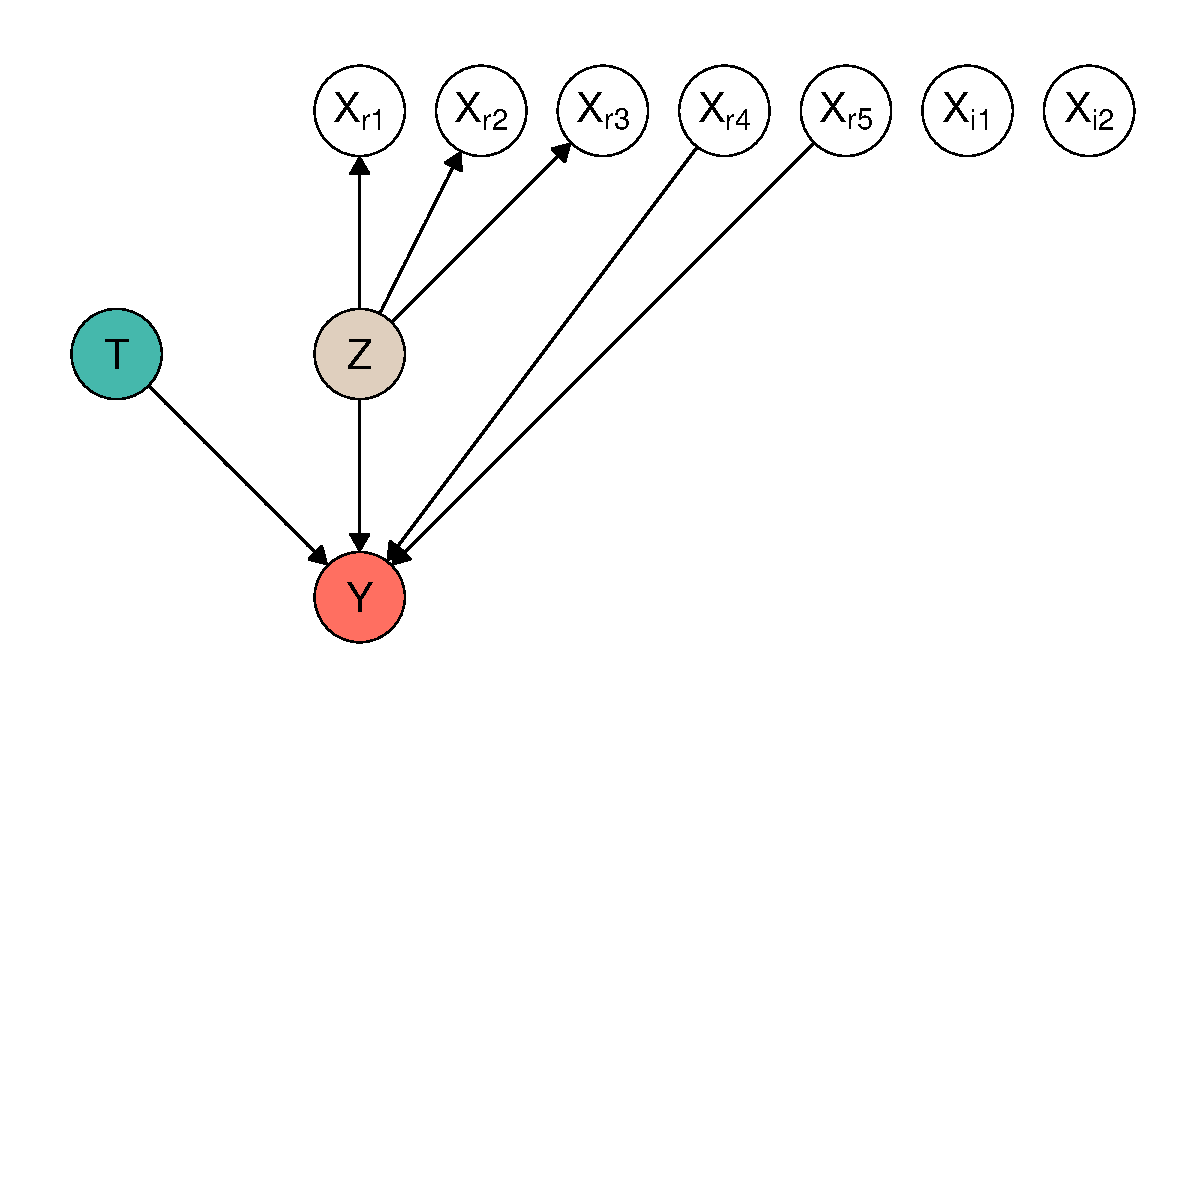
\includegraphics[width=10cm]{figs/DAG_correlated_latent.pdf}}
  
\end{frame}

% \begin{frame}{Big model vs variable selection?}

%   \begin{itemize}
%   \item If we care only about the predictive performance
%     \begin{itemize}
%     \item Include all available prior information
%     \item Integrate over all uncertainties
%     \item No need for feature selection
%     \end{itemize}
%   \item<2-> Variable selection can be useful if
%     \begin{itemize}
%     \item need to reduce measurement or computation cost in the future
%     \item improve explainability
%     \end{itemize}
%   \end{itemize}
  
% \end{frame}

\begin{frame}{Model selection is needed to avoid overfitting?}

  logistic regression: 30 \textbf{completely irrelevant} variables, \\100
  observations
  
  \only<2>{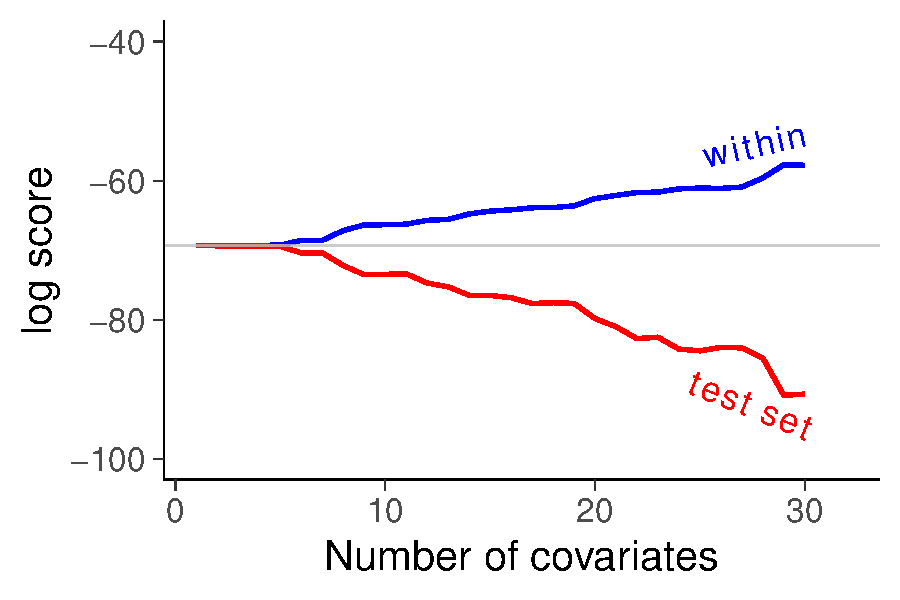
\includegraphics[width=10cm]{irrelevant_N.pdf}}

\end{frame}

\begin{frame}{Prior on parameters vs predictions}

N(0,3) prior on each coefficient\\
\only<1>{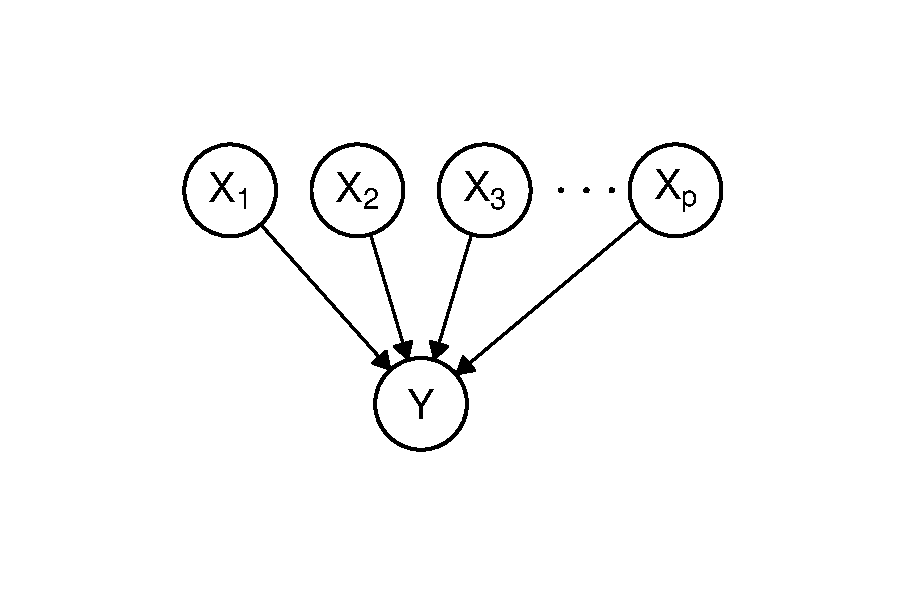
\includegraphics[width=9cm]{figs/simple.pdf}}
\only<2>{1 variable\\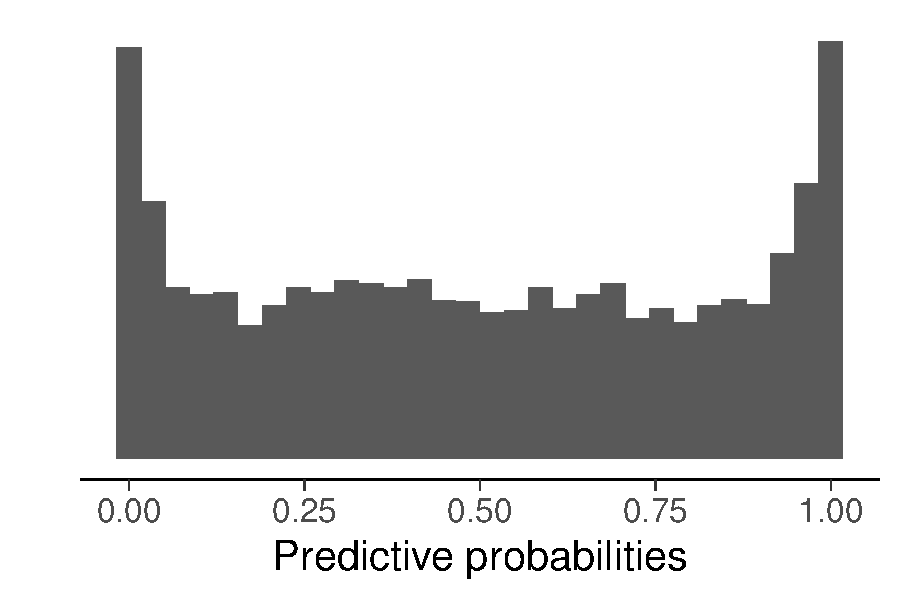
\includegraphics[width=9cm]{prior_N_1.pdf}}
\only<3>{2 variables\\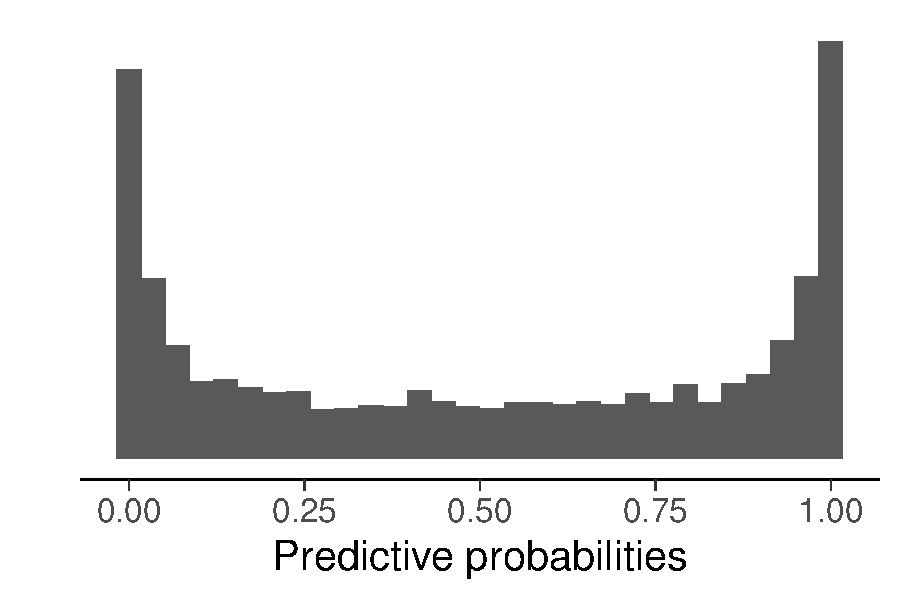
\includegraphics[width=9cm]{prior_N_2.pdf}}
\only<4>{3 variables\\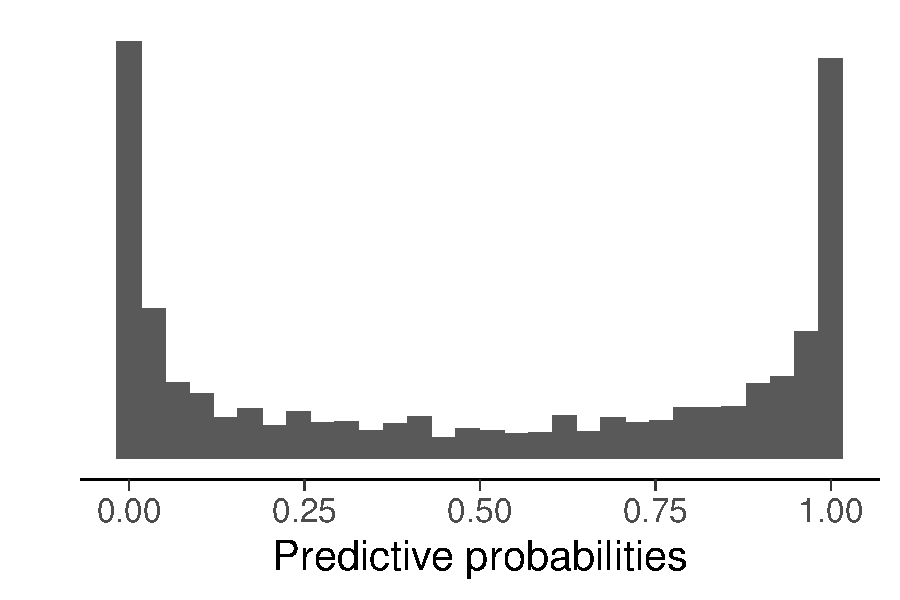
\includegraphics[width=9cm]{prior_N_3.pdf}}
\only<5-6>{30 variables\\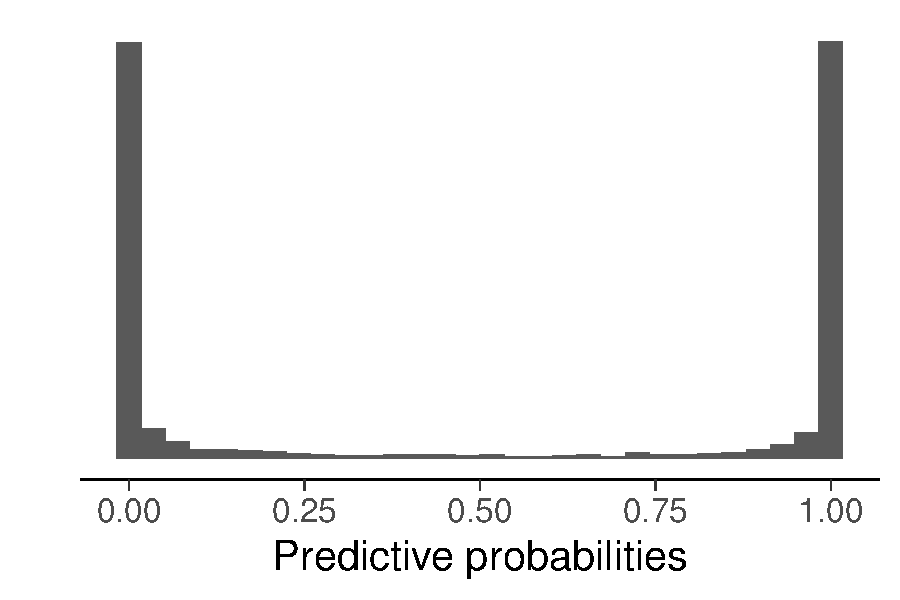
\includegraphics[width=9cm]{prior_N_30.pdf}}

\only<6>{A weak prior on parameters can be a strong prior on predictions}

\end{frame}

\begin{frame}{Better priors}

N(0,$\frac{1}{\sqrt{p}}$) prior on each coefficient\\
\only<1>{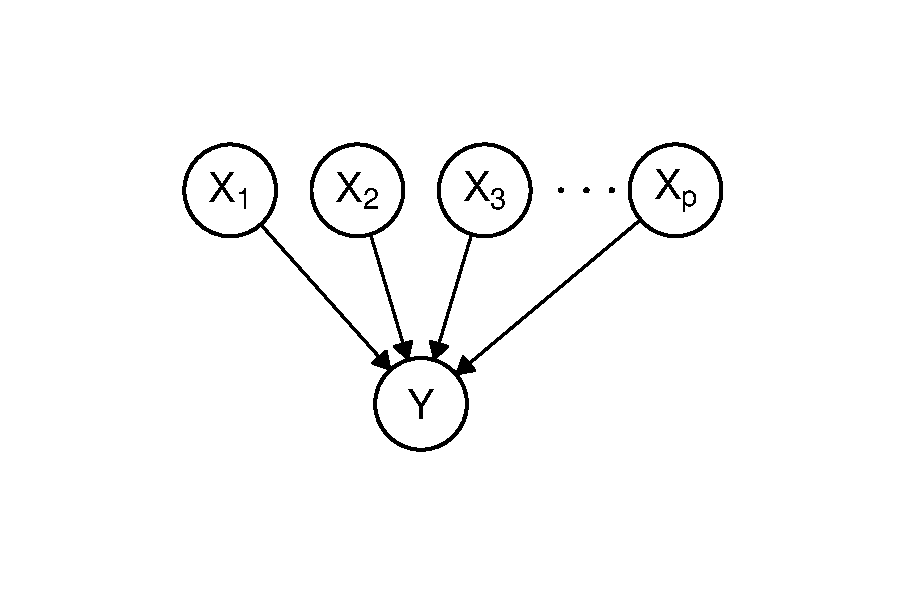
\includegraphics[width=9cm]{figs/simple.pdf}}
\only<2>{1 variable\\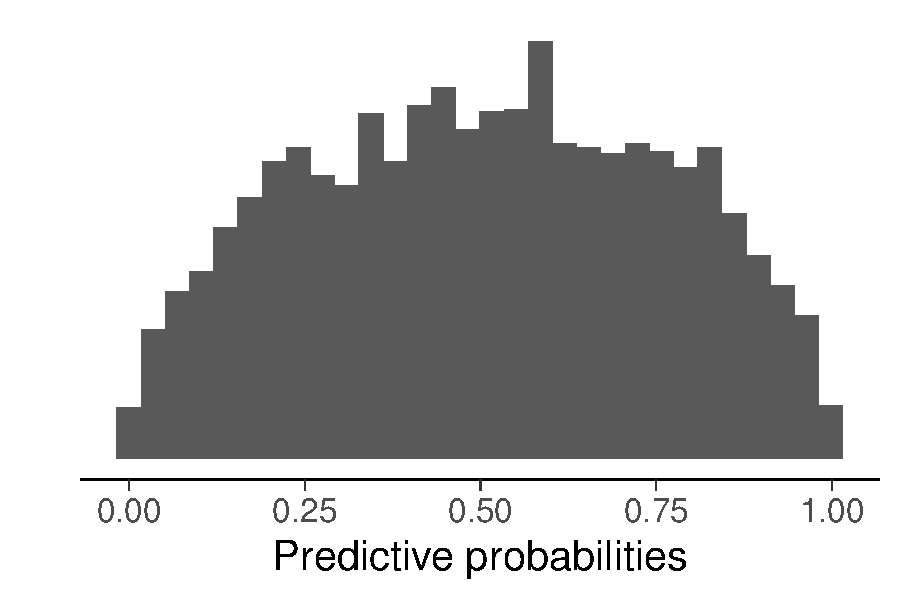
\includegraphics[width=9cm]{prior_Ns_1.pdf}}
\only<3>{2 variables\\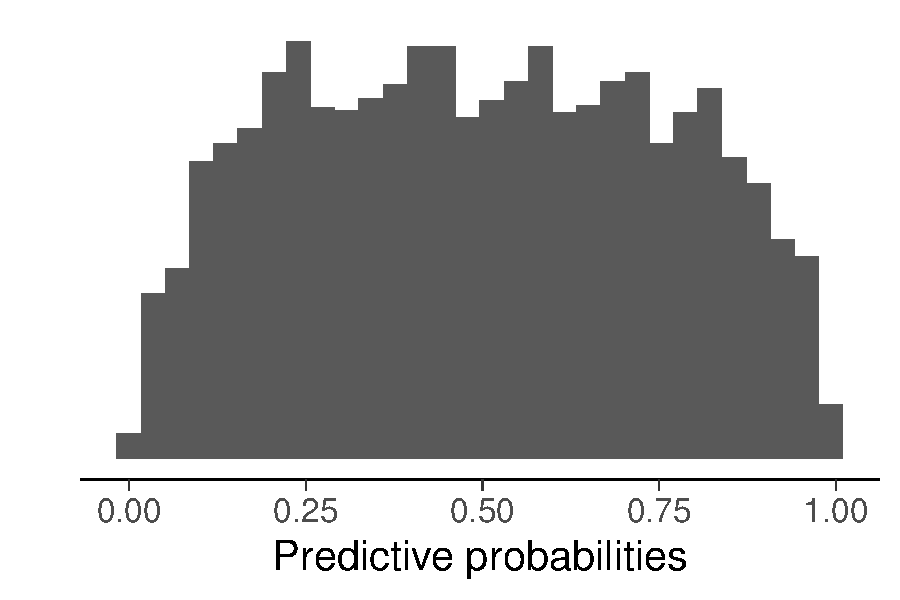
\includegraphics[width=9cm]{prior_Ns_2.pdf}}
\only<4>{3 variables\\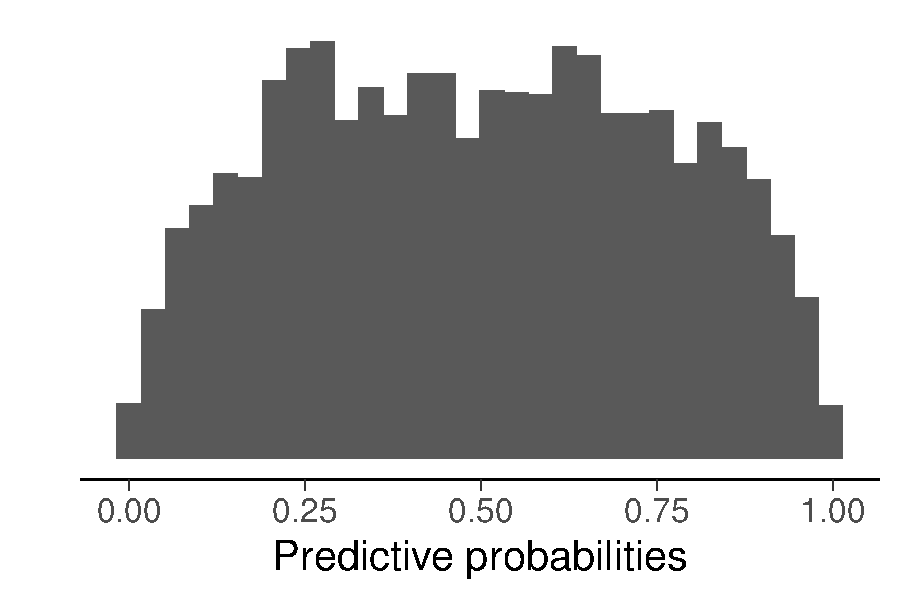
\includegraphics[width=9cm]{prior_Ns_3.pdf}}
\only<5-6>{30 variables\\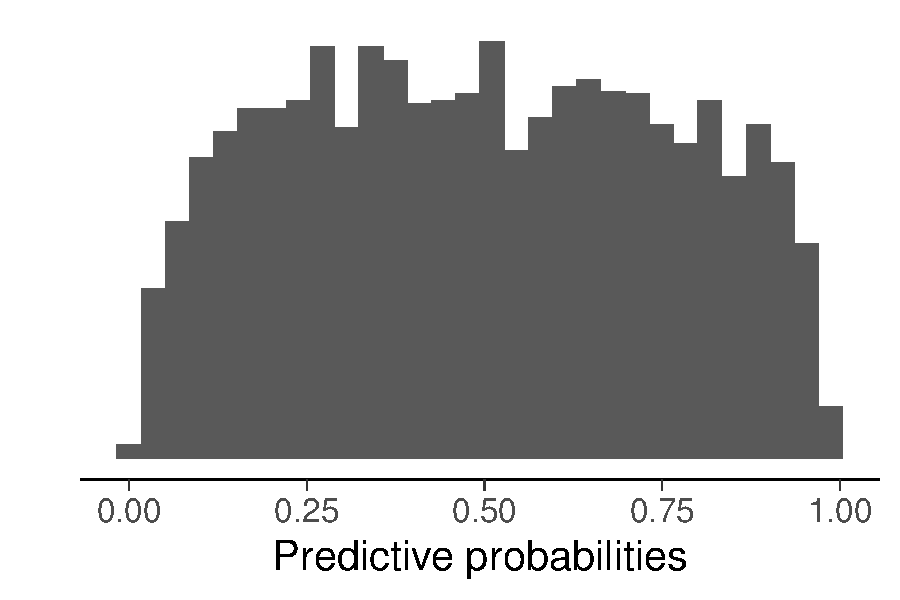
\includegraphics[width=9cm]{prior_Ns_30.pdf}}

\only<6>{Prior on predictions (almost) fixed when the model gets bigger}
  
\end{frame}

\begin{frame}{Better priors, no overfitting}

  logistic regression: 30 \textbf{completely irrelevant} variables, \\100
  observations
  
  \only<1>{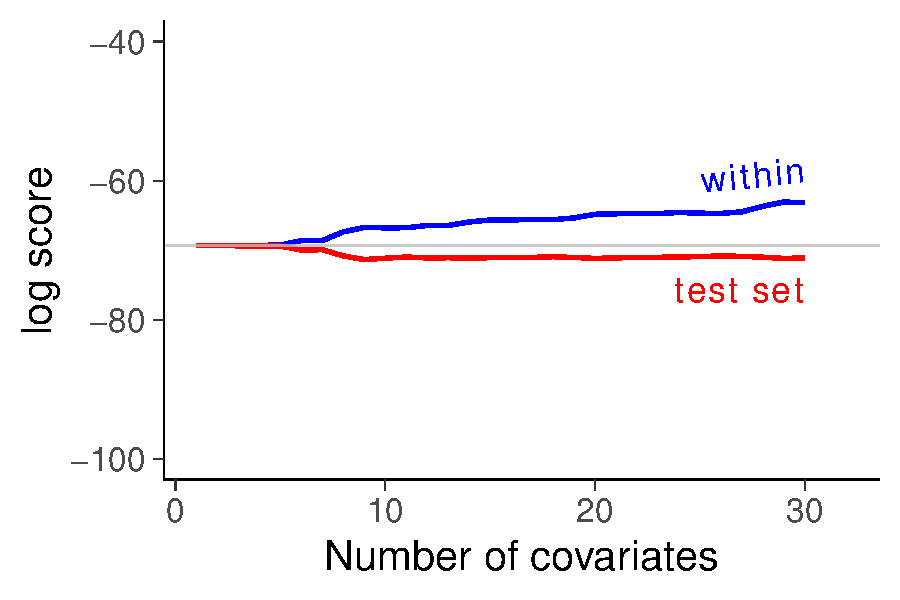
\includegraphics[width=10cm]{irrelevant_Ns.pdf}}
  \only<2>{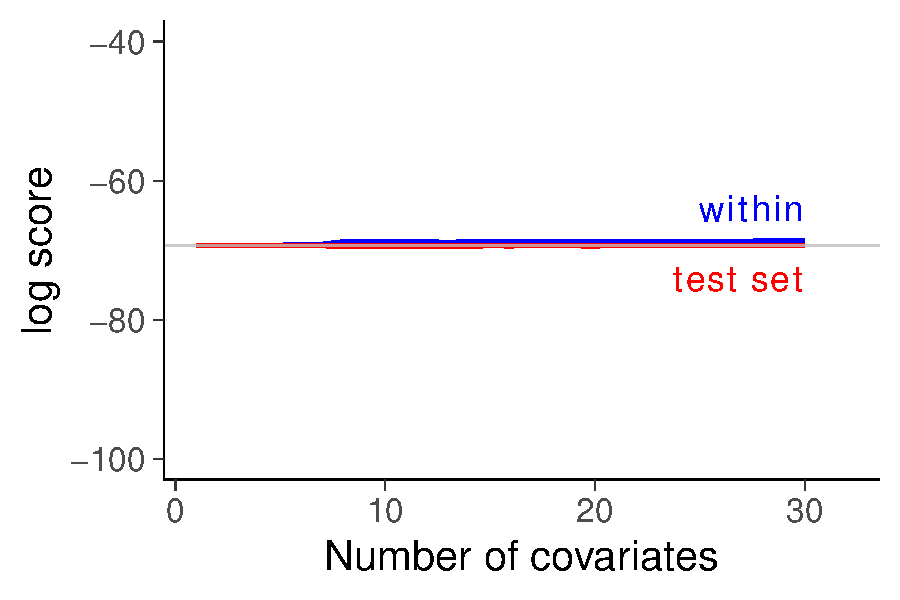
\includegraphics[width=10cm]{irrelevant_RHS.pdf}}
  
\end{frame}

\begin{frame}{Many weak effects, wide prior on parameters}

  logistic regression: 30 \textbf{weakly relevant} variables, \\100
  observations, wide prior
  
  \only<2>{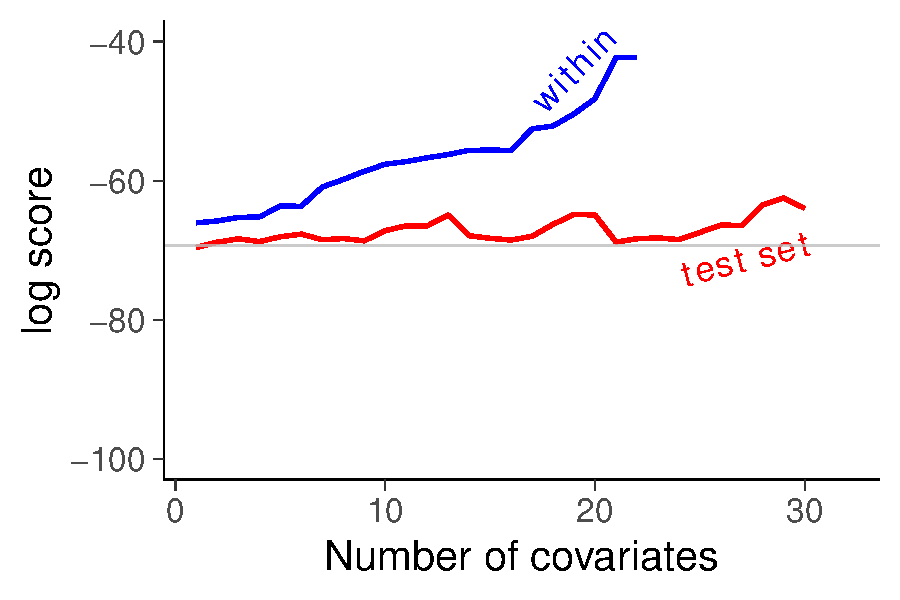
\includegraphics[width=10cm]{weak_N.pdf}}

\end{frame}

\begin{frame}{Many weak effects, better prior}

  logistic regression: 30 \textbf{weakly relevant} variables, \\100
  observations, better prior
  
  \only<1>{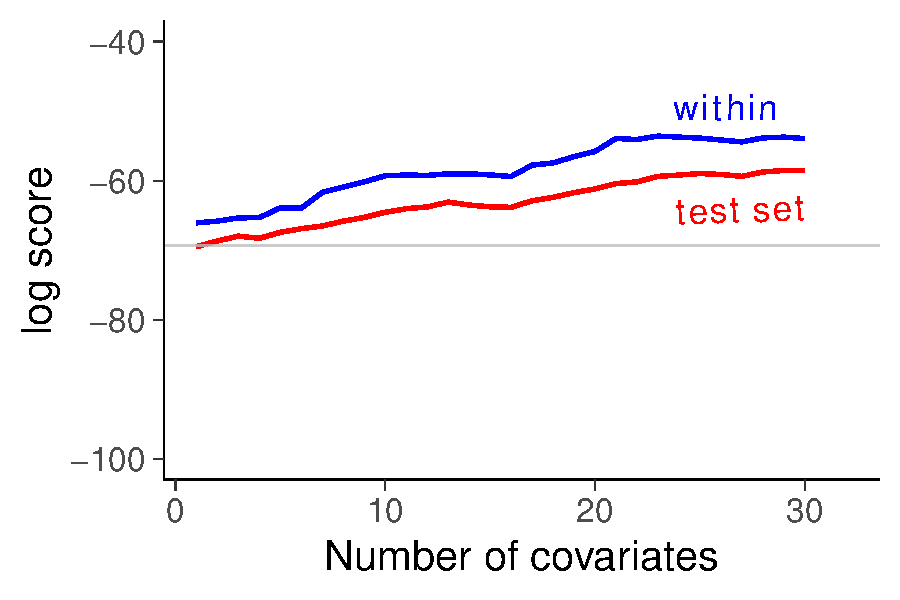
\includegraphics[width=10cm]{weak_Ns.pdf}}

\end{frame}

\begin{frame}{Correlating variables, wide prior on parameters}

  logistic regression: 30 \textbf{correlating relevant} variables, \\100
  observations
  
  % \only<1>{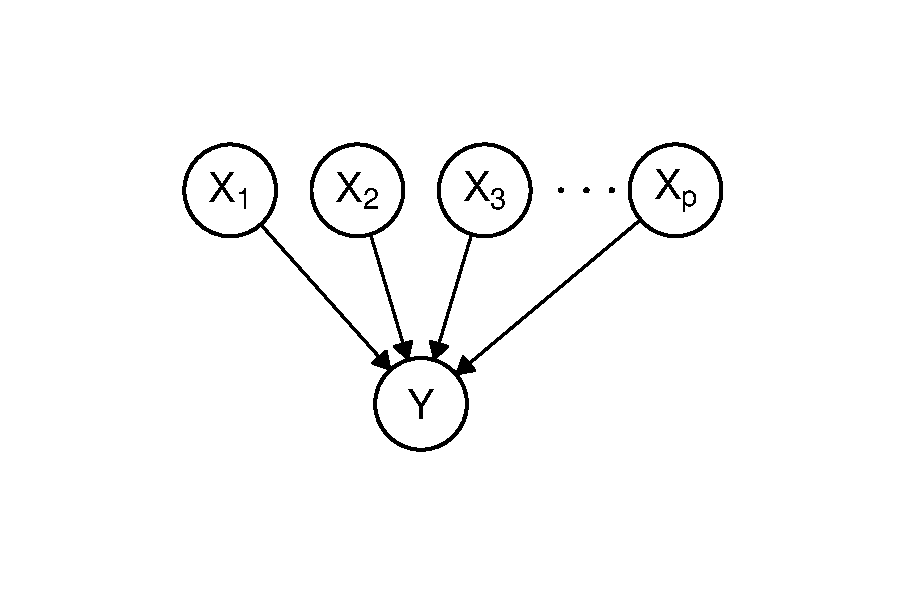
\includegraphics[width=9cm]{figs/simple.pdf}}
  \only<2>{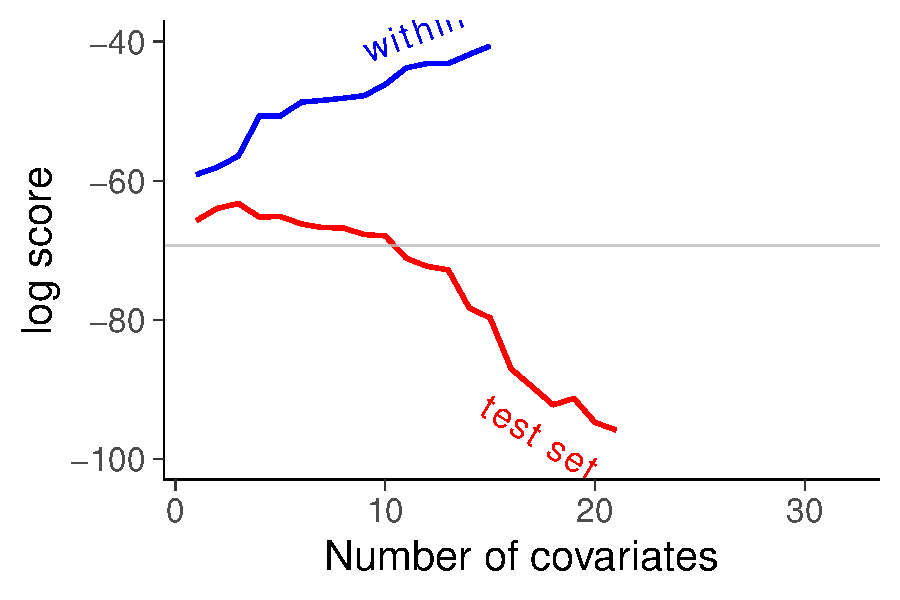
\includegraphics[width=10cm]{correlating_N.pdf}}

\end{frame}

\begin{frame}{Correlating variables, better prior}

  logistic regression: 30 \textbf{correlating relevant} variables, \\100
  observations
  
  \only<1>{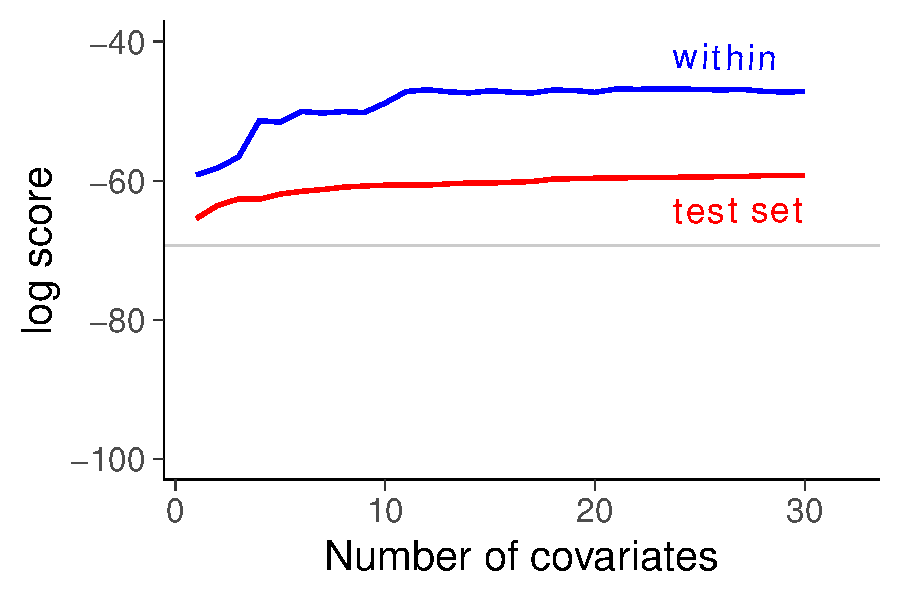
\includegraphics[width=10cm]{correlating_Ns.pdf}}

\end{frame}

\begin{frame}{Prior on $R^2$}

  Regression and Other Stories, Section 12.7 Models for regression
  coefficients: 

  \only<1>{Wide prior\\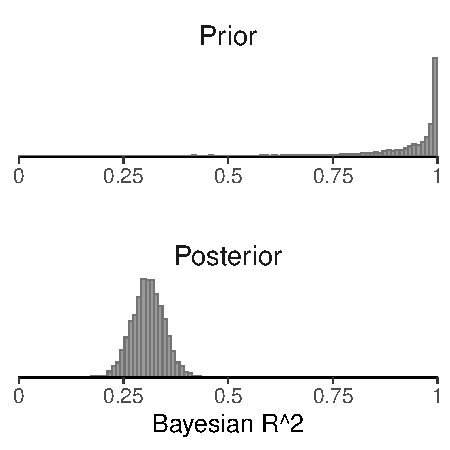
\includegraphics[width=6cm]{student_fit1_R2.pdf}}
  \only<2>{Scaled prior\\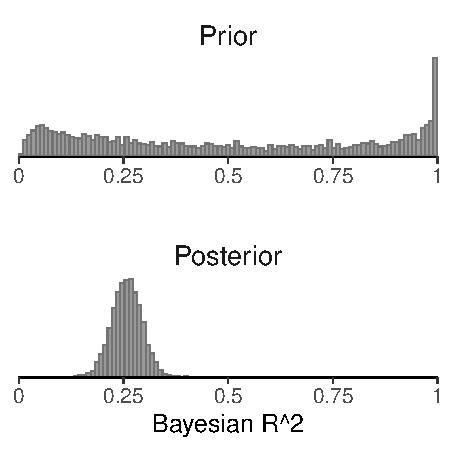
\includegraphics[width=6cm]{student_fit2_R2.pdf}}
  \only<3>{Regularized horseshoe prior\\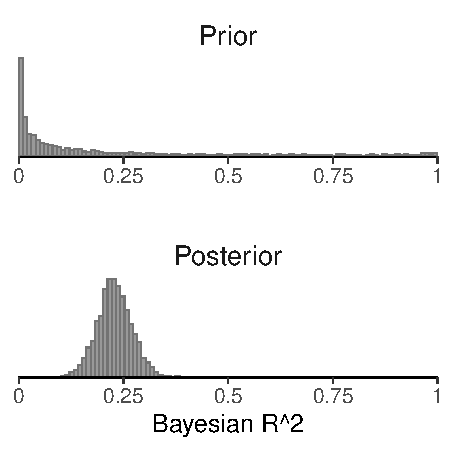
\includegraphics[width=6cm]{student_fit3_R2.pdf}}

  
\end{frame}

\begin{frame}{Better priors}

  For example:
  \begin{itemize}
  \item scaled: many weak effects
  \item regularized horseshoe, R2-D2: only some relevant
  \item R2-D2: defined directly for $R^2$
  \item PCA-type: highly correlating variables
  \end{itemize}

\end{frame}


\begin{frame}{$p \gg n$}

  \begin{itemize}
  \item With good priors, possible to have more variables than observations
  \item e.g. $p=22283, n=85$ demonstrated by Piironen, Paasiniemi,
    Vehtari (2020)
  \end{itemize}
\end{frame}


\begin{frame}{Variable selection}
  
  Variable selection
  \begin{itemize}
  \item[1.] is not needed to avoid overfitting
  \item[2.] can be used to reduce costs and improve explainability
  \end{itemize}

\end{frame}

\begin{frame}{Variable selection by looking at the posterior}

  \makebox[12.1cm][t]{
    \hspace{-0.9cm}
  \begin{minipage}[b][4cm][t]{12.1cm}
  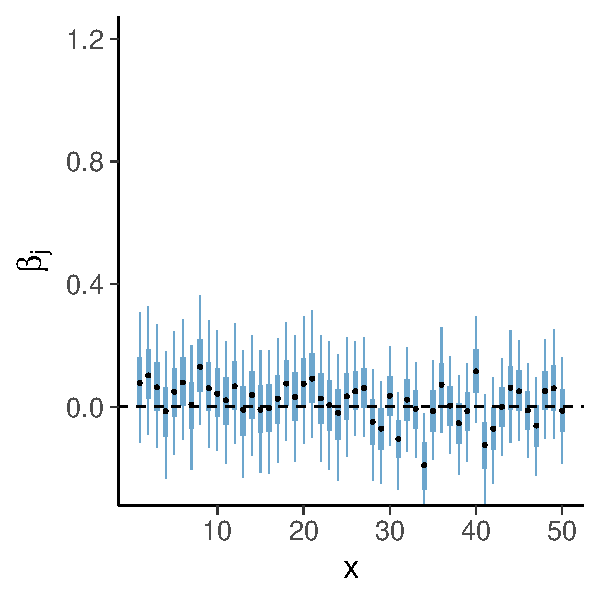
\includegraphics[width=3.9cm]{toy_marginal1.pdf}
  \uncover<2->{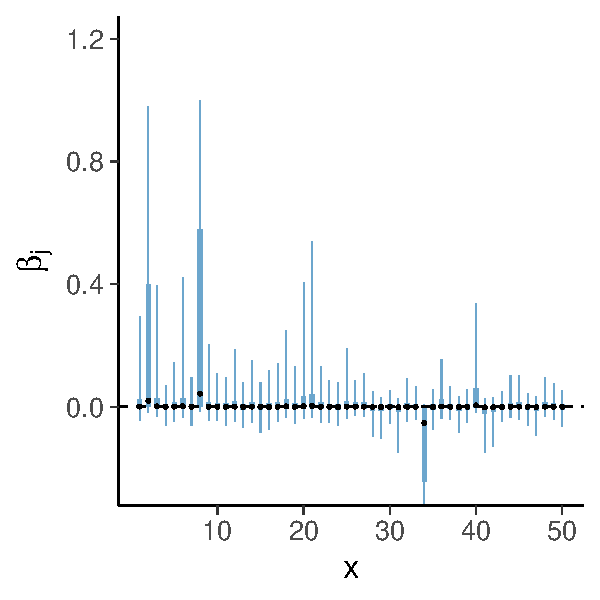
\includegraphics[width=3.9cm]{toy_marginal2.pdf}}
  \uncover<3->{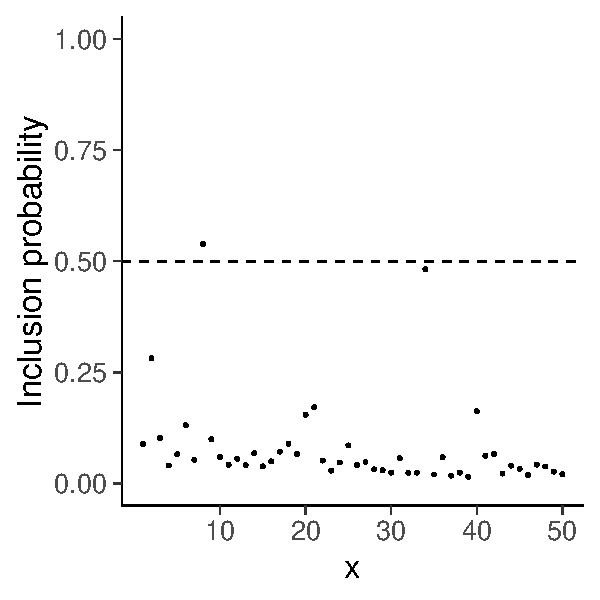
\includegraphics[width=3.9cm]{toy_marginal3.pdf}}\\
\end{minipage}
}\\
\uncover<1->{
	A) Gaussian prior, posterior median with 50\% and 90\% intervals\\ 
	}
	\uncover<2->{
	B) Horseshoe prior, same things\\ 
	}
	\uncover<3->{
	C) Spike-and-slab prior, posterior inclusion probabilities\\ 
      }
      ~\\
      \uncover<4>{25 \textbf{correlating} variables,
        25 \textbf{irrelevant} variables
% Half of the features relevant, but all marginals
% substantially overlapping with zero
}
\end{frame}

\begin{frame}{}

  {\Large\color{navyblue} What happens?}

  \makebox[12.1cm][t]{
    \hspace{-0.3cm}
    \begin{minipage}[b][8.1cm][t]{12.1cm}
      \makebox[0cm][t]{\hspace{-0.4cm}\rotatebox{90}{\hspace{1.4cm}Gaussian}}
      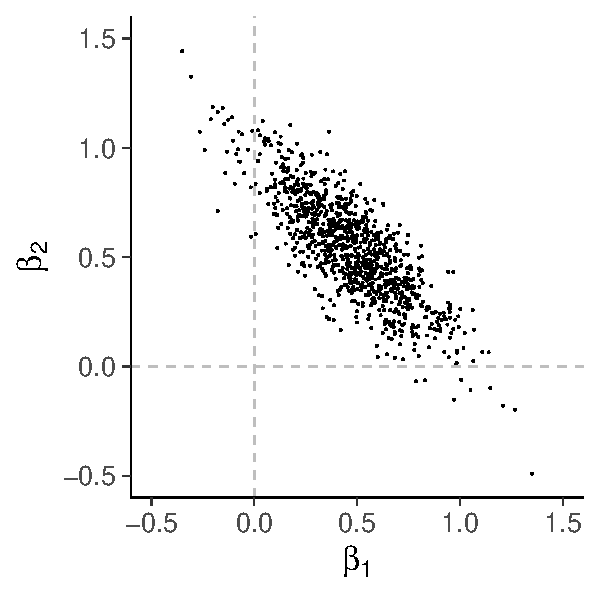
\includegraphics[width=3.7cm]{toy_scatter1.pdf}
      \uncover<2->{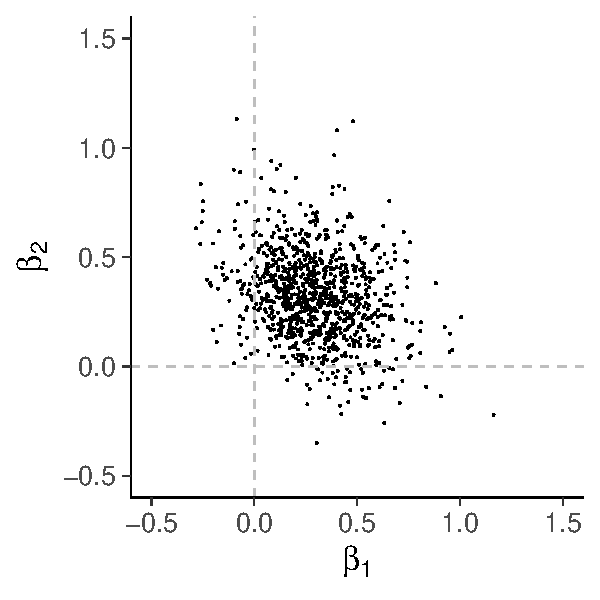
\includegraphics[width=3.7cm]{toy_scatter3.pdf}}
      \uncover<3->{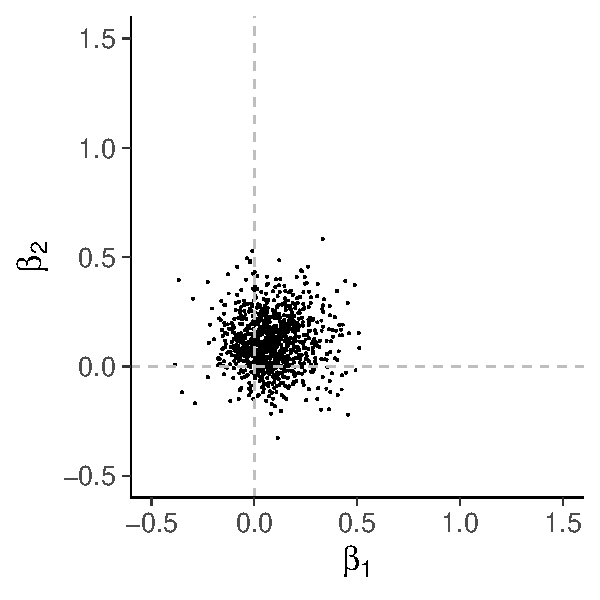
\includegraphics[width=3.7cm]{toy_scatter5.pdf}}\\
      \makebox[0cm][t]{\hspace{-0.4cm}\rotatebox{90}{\hspace{1.4cm}Horseshoe}}
      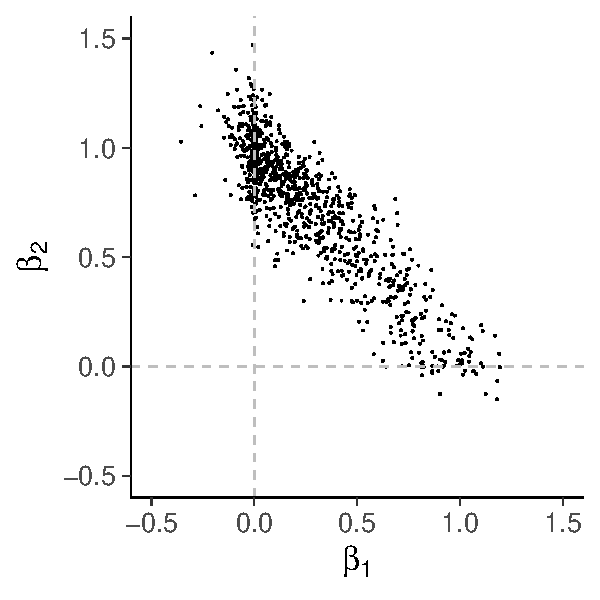
\includegraphics[width=3.7cm]{toy_scatter2.pdf}
      \uncover<2->{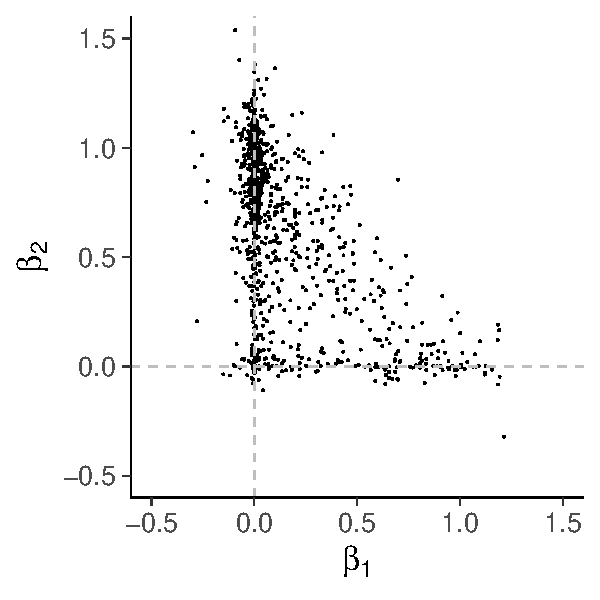
\includegraphics[width=3.7cm]{toy_scatter4.pdf}}
      \uncover<3->{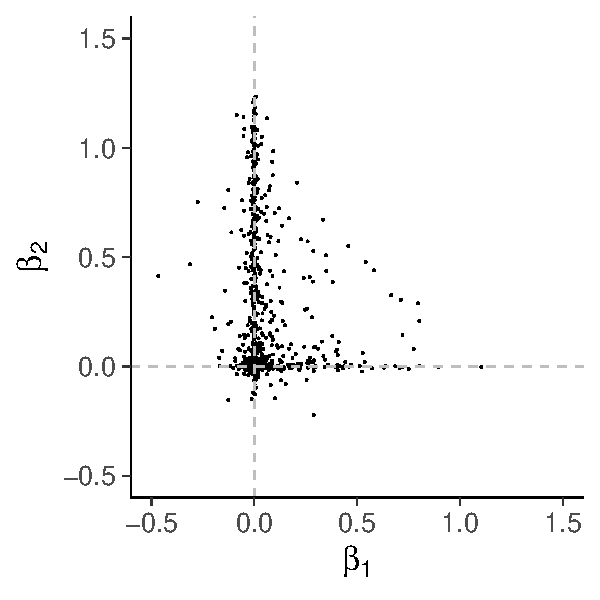
\includegraphics[width=3.7cm]{toy_scatter6.pdf}}\\
      \makebox[3.7cm]{$\quad p_\text{rel}=2$}
      \uncover<2->{\makebox[3.7cm]{$\quad p_\text{rel}=5$}}
      \uncover<3->{\makebox[3.7cm]{$\quad p_\text{rel}=25$}}
\end{minipage}
}
\end{frame}

\begin{frame}{Variable selection}

  \begin{itemize}
  \item We can do variable selection based on the predictive
    performance
  \end{itemize}

%   I'm not saying here anything about what we can infer about the coefficients
% (I'll come back to that later)

\end{frame}

\begin{frame}{Stepwise selection?}

Mix of \textbf{correlating} and \textbf{irrelevant} variables
  
  \only<2>{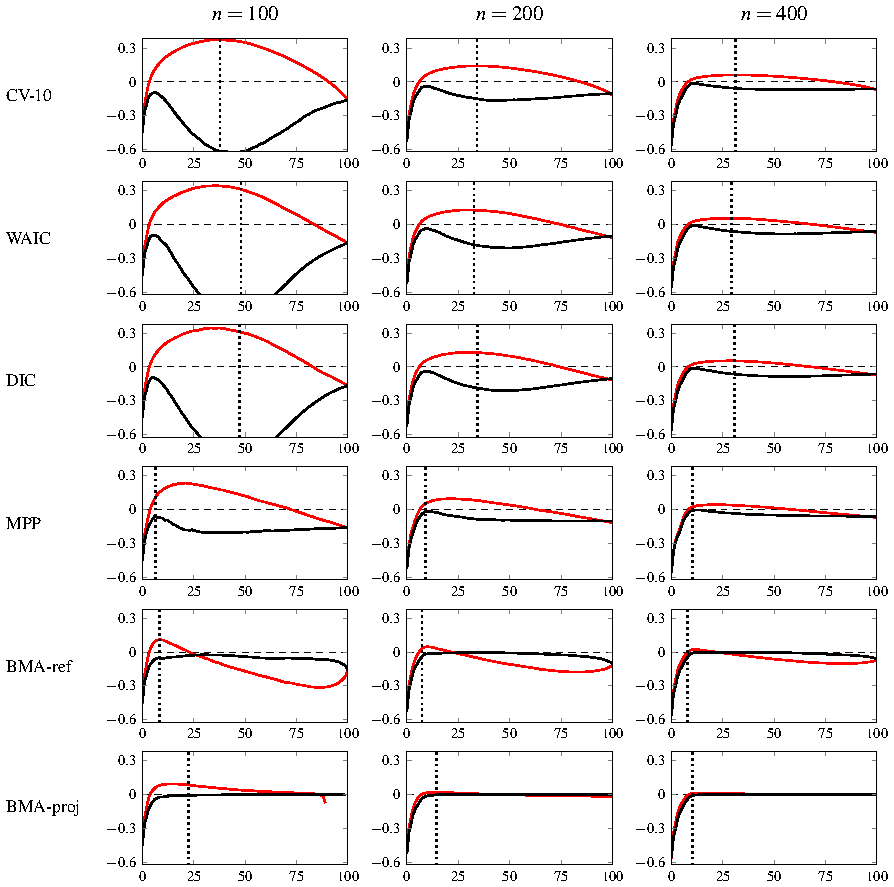
\includegraphics[width=11cm,trim=0 340 0 0,clip]{simulated_searchpath.pdf}}
  \only<3>{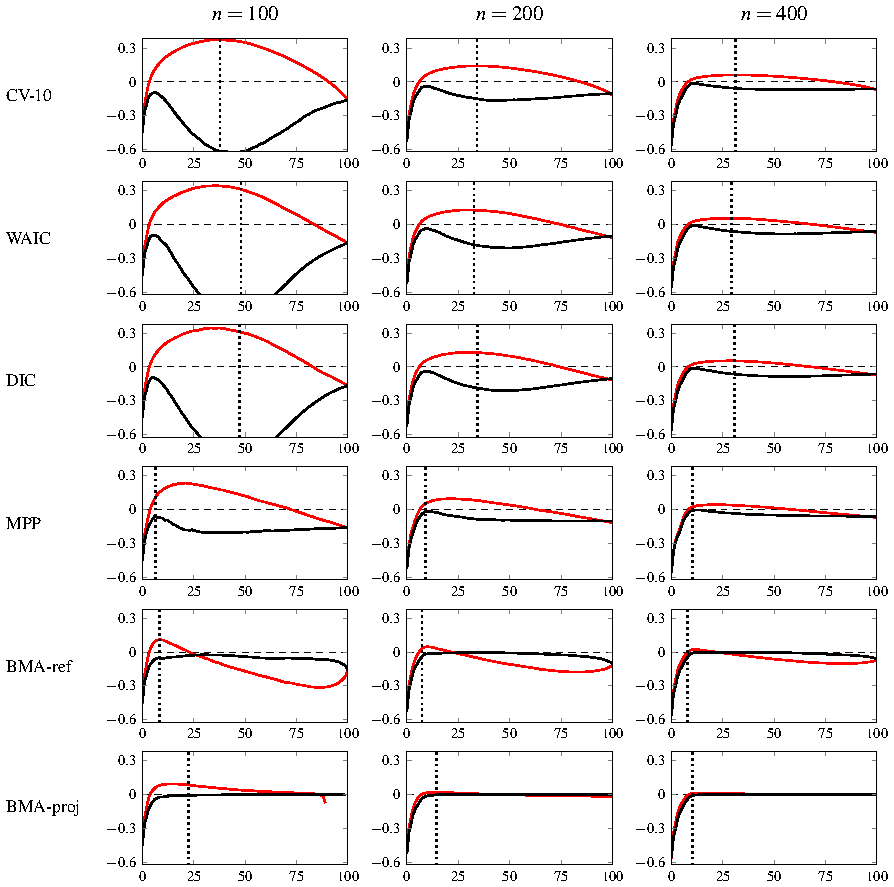
\includegraphics[width=11cm,trim=0 275 0 0,clip]{simulated_searchpath.pdf}}


\end{frame}

\begin{frame}{Reference model improves variable selection}

  Mix of \textbf{correlating} and \textbf{irrelevant} variables\\
  $n=30$, $p=500$, $p_\text{rel}=150$%, $\rho=0.5$

  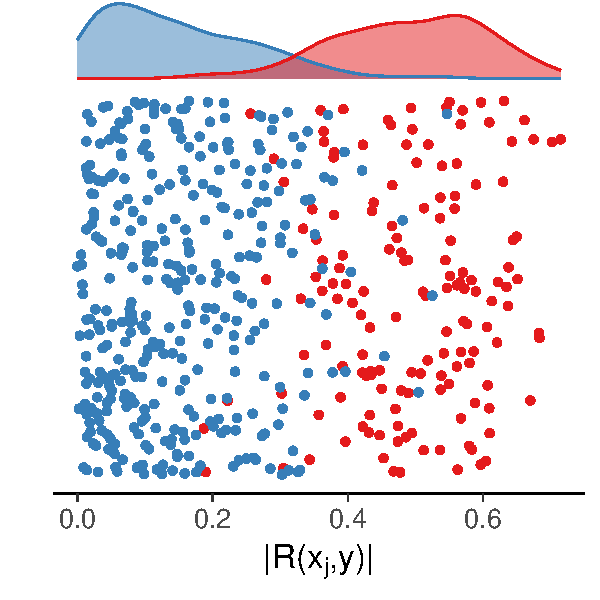
\includegraphics[width=5.5cm]{toy_corr1.pdf}\\
  \vspace{-0.2cm}
  \hspace{0.5cm} {\color{set12} irrelevant $x_j$}, {\color{set11} relevant $x_j$}\\
  \vspace{0.2cm}
  \hspace{0.5cm} Sample correlation with $y$\\
  
\end{frame}

\begin{frame}{Reference model improves variable selection}

  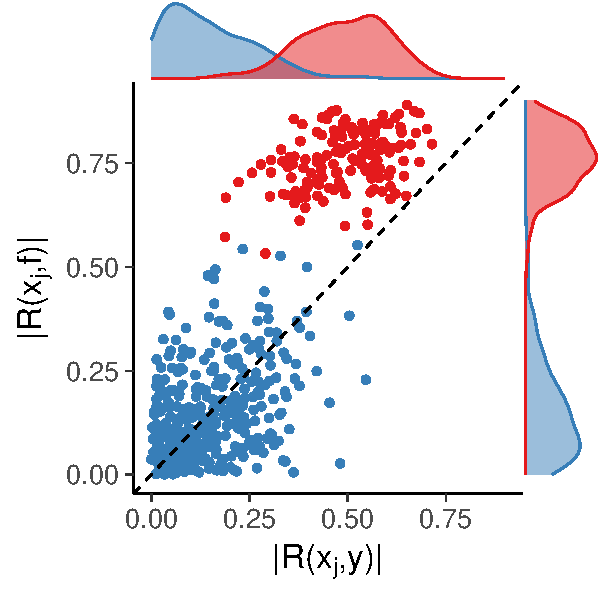
\includegraphics[width=5.3cm]{toy_corr2.pdf}
  \uncover<2->{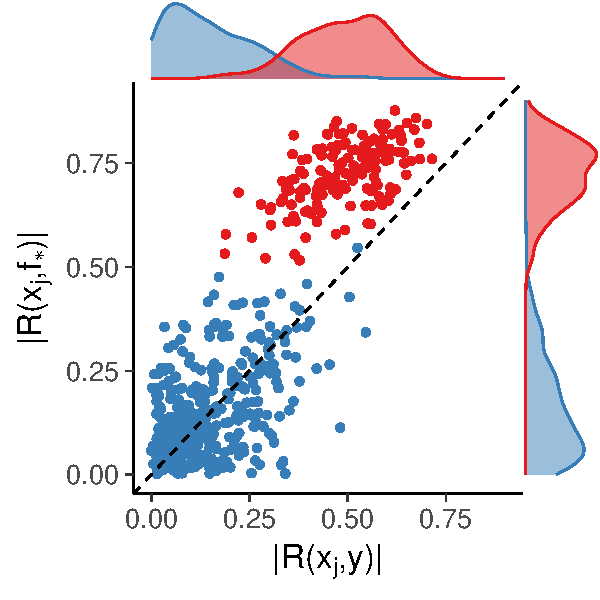
\includegraphics[width=5.3cm]{toy_corr3.pdf}}\\
  \vspace{-0.2cm}
  \hspace{0.5cm} {\color{set12} irrelevant $x_j$}, {\color{set11} relevant $x_j$}\\
  \vspace{0.2cm}
  A) Sample correlation with $y$ vs. sample correlation with $f$\\
  \uncover<2->{B) Sample correlation with $y$ vs. sample correlation with $f_*$\\
  $f_* = $ linear regression fit with 3 supervised principal components}
  
\end{frame}

%Pure noise variables are less correlated with the rich model predictions
\begin{frame}{}

  {\Large\color{navyblue} Predictive projection, idea}
  
  \begin{itemize}
  \item Model simplification technique
  \item<2-> Replace full posterior $p(\theta \mid D)$ with
    some constrained $q(\theta)$ so that the \emph{predictive
      distribution} changes as little as possible
  \item<3-> Example constraints
    \begin{itemize}
    \item $q(\theta)$ can have only point mass at some $\theta_0$ \\
      $\Rightarrow$ ``Optimal point estimates''
    \item<4-> Some features must have exactly zero regression coefficient \\
      $\Rightarrow$ ``Which features can be discarded''
    \end{itemize}
    \vspace{1\baselineskip}
  \item<5-> The decision theoretic idea of conditioning the smaller
    model inference on the full model can be tracked to Lindley (1968)
    \begin{itemize}
    \item draw by draw projection introduced by Goutis \& Robert
      (1998), and Dupuis \& Robert (2003)
    \item see also many related references in a review by
      \href{http://dx.doi.org/10.1214/12-SS102}{Vehtari \& Ojanen
        (2012)}
    \end{itemize}
\end{itemize}

\end{frame}

\begin{frame}{}

  {\Large\color{navyblue} Logistic regression with two features}

  \vspace{\baselineskip}
  
  \begin{overlayarea}{\textwidth}{0.7\textwidth}
    \begin{minipage}{0.99\textwidth}
      \begin{center}
        \only<1>{ \minput{proj_posterior} }%
        \only<2>{ \minput{proj_b1b2_single} }%
        \only<3>{ \minput{proj_b2_single} }%
        \only<4>{ \minput{proj_b1_single} }%
        \only<5>{ \minput{proj_b2_dbd} }%
        \only<6>{ \minput{proj_b1_dbd} }%
      \end{center}
    \end{minipage}
    \begin{minipage}{0.99\textwidth}
      \only<1>{Full posterior for $\beta_1$ and $\beta_2$ and contours of predicted class probability}
      \only<2>{Projected point estimates for $\beta_1$ and $\beta_2$}
      \only<3>{Projected point estimates, constraint $\beta_1 = 0$}
      \only<4>{Projected point estimates, constraint $\beta_2 = 0$}
      \only<5>{Draw-by-draw projection, constraint $\beta_1 = 0$}
      \only<6>{Draw-by-draw projection, constraint $\beta_2 = 0$}
    \end{minipage}
  \end{overlayarea}
\end{frame}

\begin{frame}

  {\Large\color{navyblue} Predictive projection}


  \begin{itemize}
  \item Replace full posterior $p(\theta \mid D)$ with some
    constrained $q(\theta)$ so that the \emph{predictive distribution}
    changes as little as possible
  \item<2-> As the full posterior $p(\theta \mid D)$ is projected to $q(\theta)$
    \begin{itemize}
    \item the prior is also projected and there is no need to define
      priors for submodels separately
    \item<3-> even if we constrain some coefficients to be $0$, the
      predictive inference is conditoned on the information related
      features contributed to the reference model
    \end{itemize}
  \end{itemize}

  
\end{frame}

\frame{

  {\Large\color{navyblue} Projective selection}

\begin{itemize}
	\item How to select a feature combination? \pause
	\item For a given model size, choose feature combination with minimal projective loss \pause
	\item Search heuristics, e.g. 
	\begin{itemize}
        \item Monte Carlo search
        \item Forward search
        \item $L_1$-penalization (as in Lasso)
	\end{itemize} \pause 
      \item Use cross-validation to select the appropriate model size
        \begin{itemize}
        \item need to cross-validate over the search paths
        \end{itemize}
      \end{itemize} 
}

\begin{frame}{Stepwise selection}

  \vspace{-0.5\baselineskip}
Mix of \textbf{correlating} and \textbf{irrelevant} variables
  
%  \only<1>{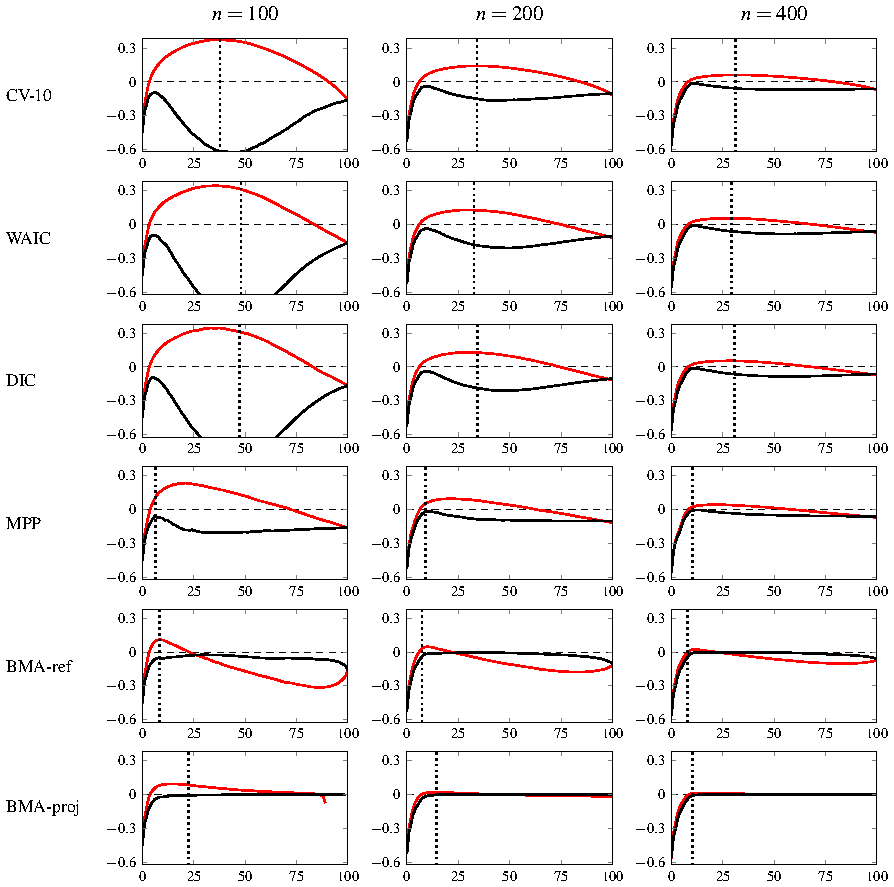
\includegraphics[width=11cm,trim=0 340 0 0,clip]{simulated_searchpath.pdf}}
  \only<1->{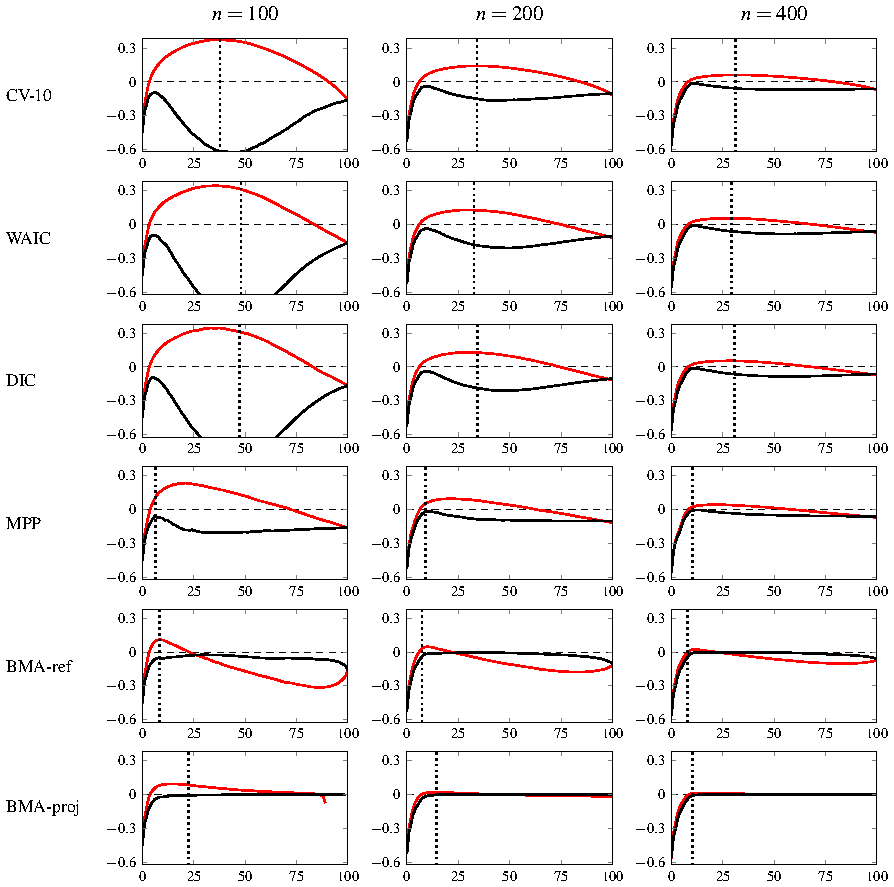
\includegraphics[width=11cm,trim=0 275 0 0,clip]{simulated_searchpath.pdf}}
  \only<2->{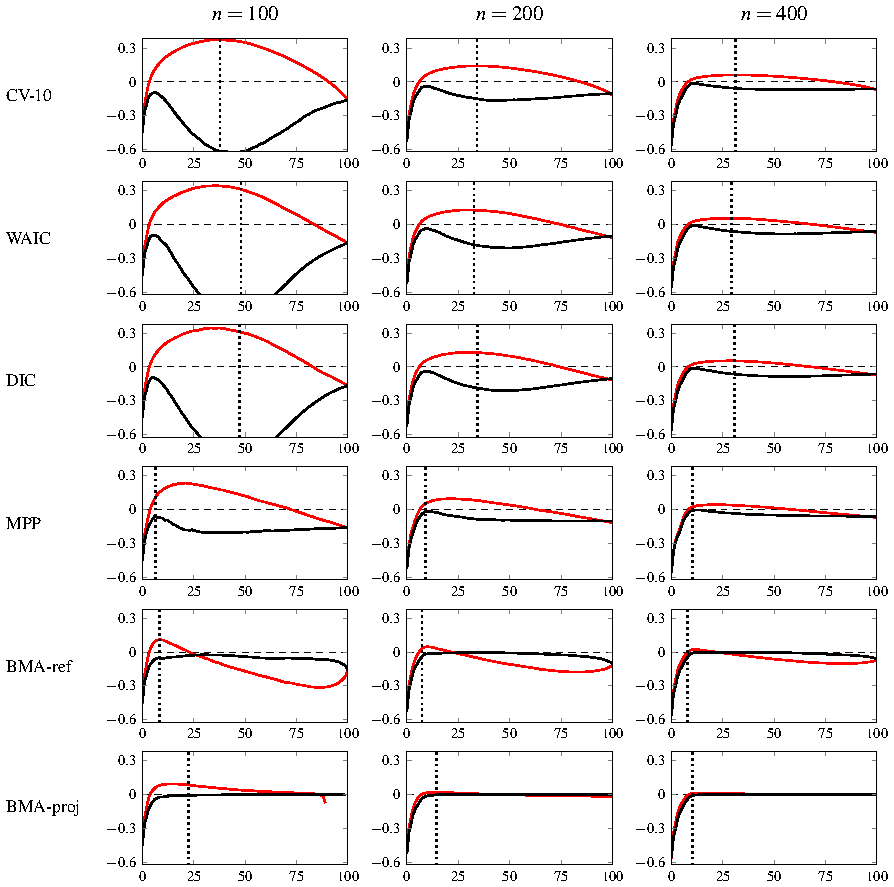
\includegraphics[width=11cm,trim=0 68 0 290,clip]{simulated_searchpath.pdf}}
  \only<3>{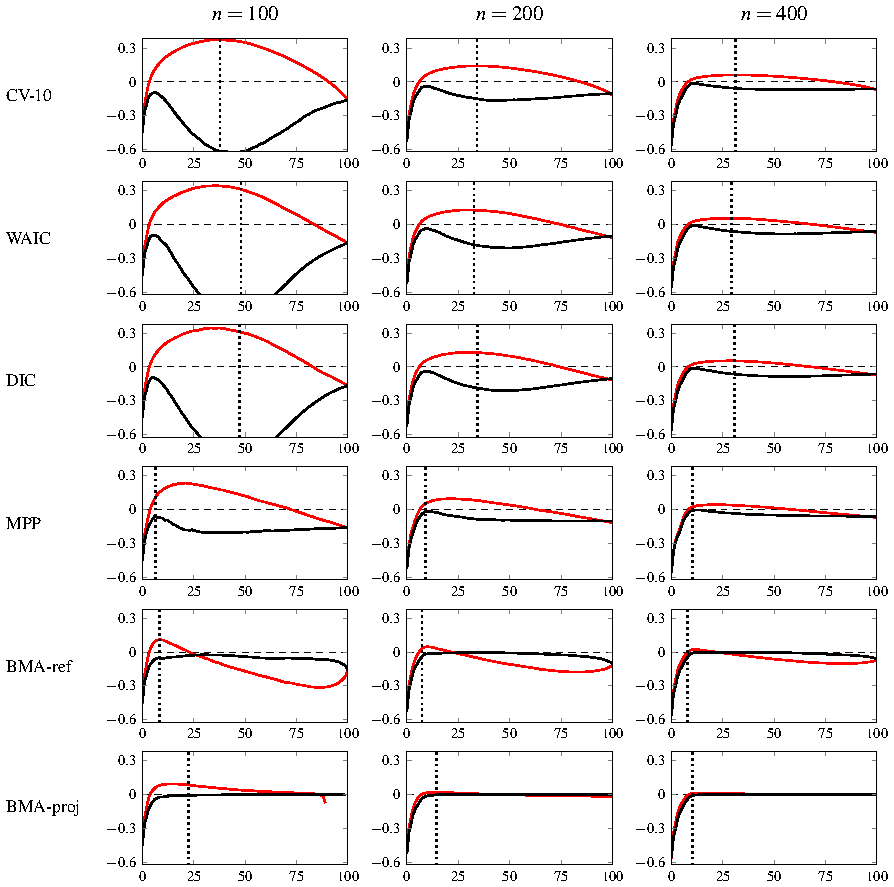
\includegraphics[width=11cm,trim=0 0 0 360,clip]{simulated_searchpath.pdf}}


\end{frame}

\frame{

  {\Large\color{navyblue} Projective selection vs. Lasso}

Same simulated regression data as before, \\
$n=50$, $p=500$, $p_\text{rel} = 150$, $\rho=0.5$

\vspace{0.5em}

  \makebox[12.1cm][t]{
    \hspace{-0.5cm}
  \begin{minipage}{0.99\textwidth}
      \only<1>{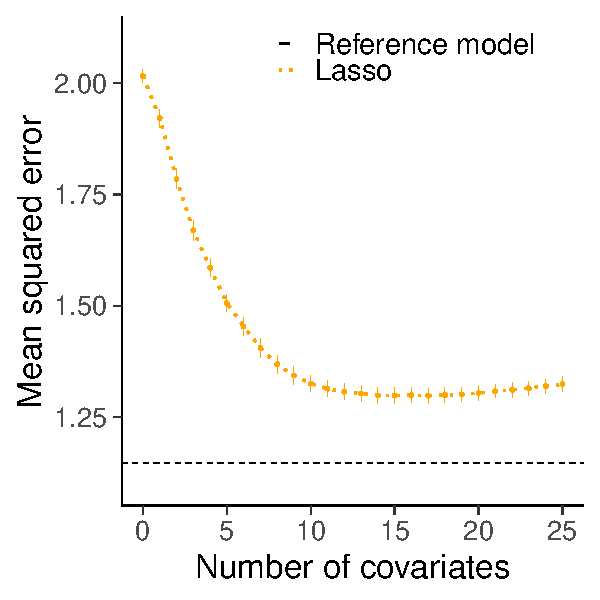
\includegraphics[width=5.5cm]{vslasso1rmse.pdf}}
      \only<2>{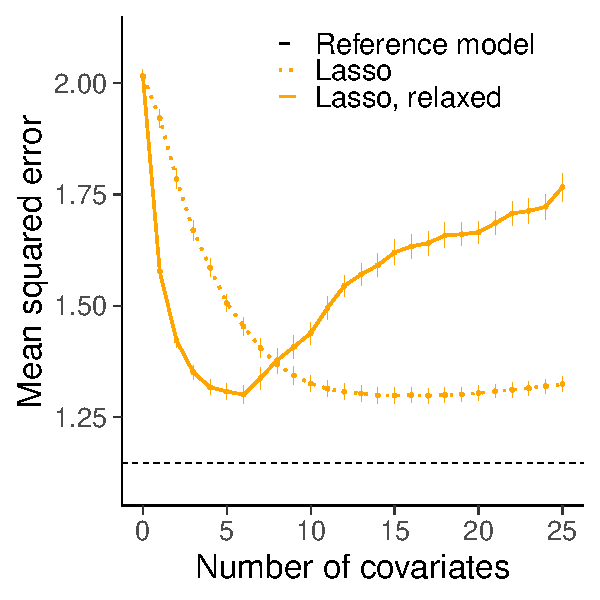
\includegraphics[width=5.5cm]{vslasso2rmse.pdf}}
      \only<3->{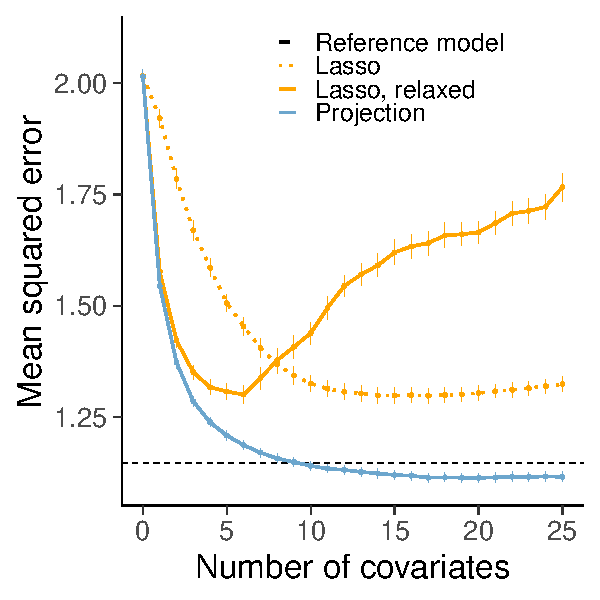
\includegraphics[width=5.5cm]{vslasso3rmse.pdf}}
      \uncover<4>{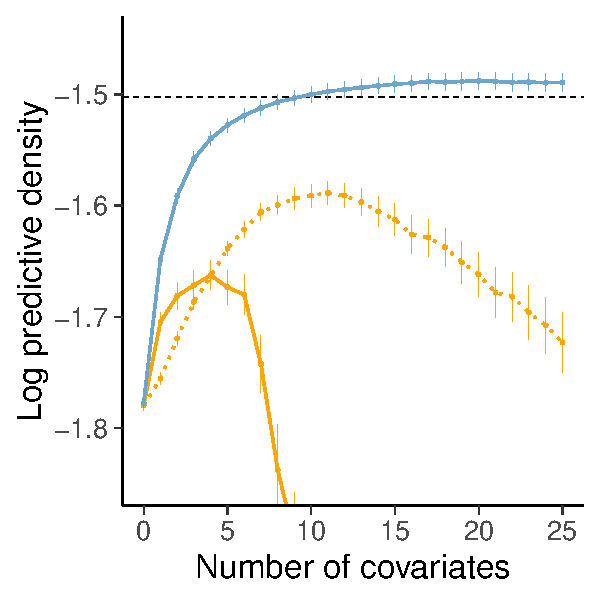
\includegraphics[width=5.5cm]{vslasso3mlpd.pdf}}
  \end{minipage}
  }
  
}

\begin{frame}{Reference model improves variable selection}

  \begin{itemize}
  \item Use of a reference model can improve even stepwise selection
  \item Projection predictive approach even better
  \end{itemize}

\end{frame}

\begin{frame}{Projection predictive inference}

  \begin{itemize}
  \item Project the reference model posterior to the parameter space
    of a smaller model
  \item Choose the smallest model with similar predictive performance
    as the reference model
  \item<2-> Improves the selection process and provides good predictions
    after the selection
  \end{itemize}

\end{frame}

\begin{frame}{Bodyfat example}

  \vspace{-0.55\baselineskip}
  Predict bodyfat percentage. The reference value is obtained by
  immersing person in water. $n=251$.

  \pause
  \vspace{-0.7\baselineskip}
  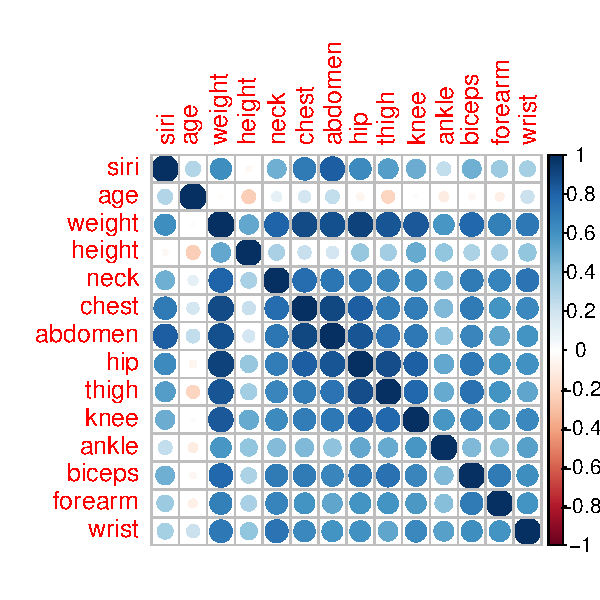
\includegraphics[width=7.7cm]{bodyfat_corr.pdf}

\end{frame}

\begin{frame}{Bodyfat}

  \vspace{-0.55\baselineskip}
  Marginal posteriors of coefficients
  
  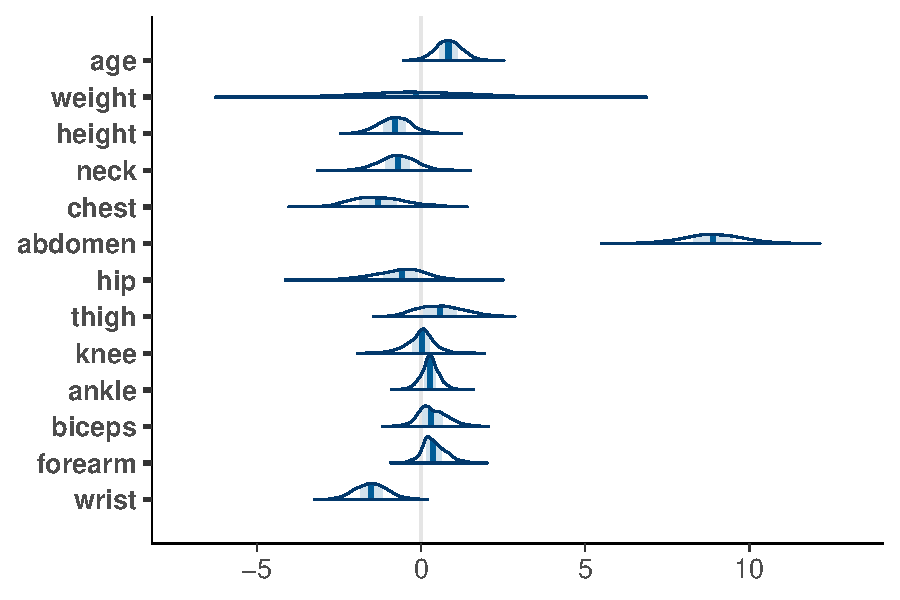
\includegraphics[width=11cm]{bodyfat_mcmc_areas.pdf}

\end{frame}

\begin{frame}{Bodyfat}

  \vspace{-0.55\baselineskip}
  Bivariate marginal of weight and height
  
  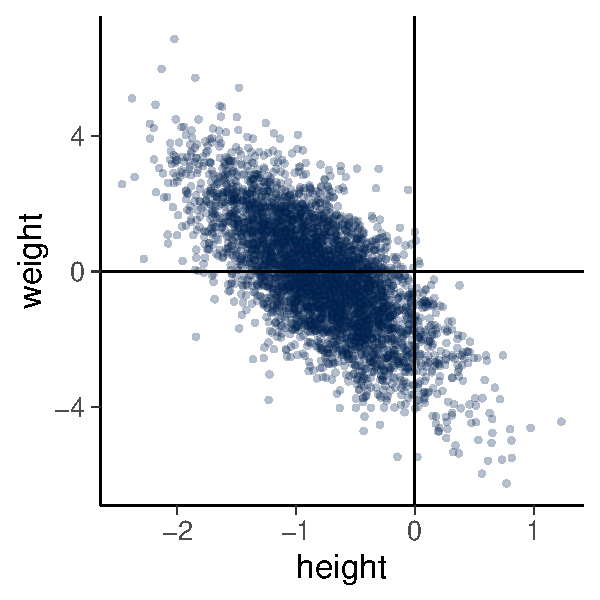
\includegraphics[width=7.5cm]{bodyfat_mcmc_scatter.pdf}

\end{frame}

\begin{frame}{Bodyfat}

  \vspace{-0.55\baselineskip}
  The predictive performance of the full and submodels
  
  \includegraphics[width=11cm]{bodyfat_varsel_plot.pdf}

\end{frame}


\begin{frame}{Bodyfat}

  \vspace{-0.55\baselineskip}
  Marginals of projected posterior
  
  \includegraphics[width=11cm]{bodyfat_proj_mcmc_areas.pdf}

\end{frame}

\begin{frame}{Bodyfat}

  \vspace{-0.55\baselineskip}
  Inclusion probabilities in bootstrap simulation\\
  \texttt{projpred} vs \texttt{steplm}

  \uncover<2->{
  \hspace{-1cm}
  \begin{minipage}[t][\arraycolsep][t]{1.0\linewidth}
    \includegraphics[width=12.5cm,trim=0 0 70 0,clip]{inc_prob.pdf}
  \end{minipage}
  \\
  \hspace{1cm}\includegraphics[height=2cm,trim=650 70 0 70,clip]{inc_prob.pdf}
}

  \vspace{-1.5\baselineskip}
  \begin{itemize}
  \item<3> In case of highly correlating variables and finite data, there
    will be variation in the selected variables
  \end{itemize}

  
\end{frame}

\begin{frame}{Reference models in variable selection}

  Reference models
  \begin{itemize}
  \item[3.] improve stability and reduces overfitting in selection
  \item[4.] projection of the reference model is even better
  \end{itemize}

\end{frame}

\begin{frame}{Inference after selection?}

  \begin{itemize}
  \item For example, for inference on treatment effect, it's best to
    use the big good model
  \item Under certain conditions, the projected posterior is also well
    calibrated, but we're still investigating more details
  \end{itemize}

\end{frame}

\begin{frame}{Beyond simple regression}

  \begin{itemize}
  \item We have implemented projection predictive approach for
    \begin{itemize}
    \item generalized linear models (also non-exponential family)
    \item hierarchical models
    \item splines
    \item Gaussian processes
    \end{itemize}
  \item<2-> The reference model approach can be used for any models
    and with any inference
    \begin{itemize}
    \item e.g. trees and neural networks
    \end{itemize}
  \end{itemize}

\end{frame}

\begin{frame}{Software for projection predictive variable/model selection}

  \begin{itemize}
  \item \texttt{projpred} R package (in CRAN + github)
  \item \texttt{kulprit} Python package (\url{github.com/yannmclatchie/kulprit})
  \end{itemize}

\end{frame}

\begin{frame}{Reference models in variable selection}

  Variable / model selection
  \begin{itemize}
  \item[1.] is not needed to avoid overfitting
  \item[2.] can be used to reduce costs and improve explainability
  \end{itemize}

  Reference models
  \begin{itemize}
  \item[3.] improve stability and reduce overfitting in selection
  \item[4.] projection of the reference model is even better
  \end{itemize}

  Calibrated causal inference
  \begin{itemize}
  \item[5.] variable selection needs
    to take into account the causal assumptions
  \end{itemize}

\end{frame}

\begin{frame}{References and more results}

  \vspace{-1\baselineskip}
  {\footnotesize
  \begin{itemize}
  \item More results projpred vs. marginal posterior probabilities:\\
    Piironen and Vehtari (2017). Comparison of Bayesian predictive
    methods for model selection. Statistics and Computing,
    27(3):711-735.
  \item More results projpred vs. Lasso and elastic net:\\
    Piironen, Paasiniemi, Vehtari (2020). Projective inference in
    high-dimensional problems: prediction and feature selection.
    \textit{Electronic Journal of Statistics}, 14(1):2155--2197.
  \item More results on frequency properties and generic benefit of reference models:\\
    Pavone, Piironen, Bürkner, Vehtari (2022). Using reference models
    in variable selection.  \textit{Computational Statistics},
    doi:10.1007/s00180-022-01231-6.
  \item Hierarchical and spline models: \\
    Catalina, Bürkner, and Vehtari (2022). Projection predictive
    inference for generalized linear and additive multilevel
    models. AISTATS 2022, PMLR 151:4446–4461.
  % \item projpred for Gaussian graphical models:\\
  %   Williams, Piironen, Vehtari, Rast (2018). Bayesian estimation of Gaussian graphical models with projection predictive selection. \href{https://arxiv.org/abs/1801.05725}{arXiv:1801.05725}
  % \item More results for Bayes SPC:\\
  %   Piironen and Vehtari (2018). Iterative supervised principal components. 21st AISTATS, PMLR 84:106-114. \href{http://proceedings.mlr.press/v84/piironen18a.html}{Online}.
  \item More references, and several case studies for small to moderate dimensional ($p=4 \ldots 100$) small data:\\
    \url{https://avehtari.github.io/modelselection/}
  \end{itemize}
  }
\end{frame}

\end{document}

%The reference model variable selection is overfitting less to the data as the target is the refence model


%Projection briefly explained

% Prediction is easier than selecting "true variables"

% Bodyfat example

% When there are small coefficients variable selection may drop out some variables with negligible effect in the predictive performance 

% When there are correlating variables, variable selection may drop out some variables with negligible effect in the predictive performance 

% Thus with realistic simulations there is likely to be some variation in which variables are included

% Refence model reduces that variability anyway

% Due to the possible small effects and correlations, we can find a
% minimal set with good predictive performance, but more difficult to
% find all

% projpred, given some constraint how to project the posterior to the constraint space and ...

Inference after selection?

On going work

%%% Local Variables: 
%%% mode: latex
%%% TeX-master: t
%%% End:
